% !TeX spellcheck = russian-aot-ieyo
% Зачем: Определяет класс документа (То, как будет выглядеть документ)
% Примечание: параметр draft помечает строки, вышедшие за границы страницы, прямоугольником, в фильной версии его нужно удалить.
\documentclass[a4paper,14pt,russian,oneside,final]{extreport}

% Зачем: Предоставляет проприетарный Times New Roman.
% ОБНОВЛЕНИЕ: лучше использовать scalable-cyrfonts-tex: меньше проблем с установкой
% Из руководства к PSCyr: "Во избежание проблем пакет PSCyr должен загружаться перед пакета-ми inputenc и babel".
% Примечание: Требует шаманства при установке, инструкция http://plumbum-blog.blogspot.com/2010/06/miktex-28-pscyr-04d.html
% http://blog.harrix.org/?p=444
% надо закомментировать это, чтобы использовать scalable-cyrfonts-tex:
% \usepackage{pscyr}

% Зачем: Делает результирующий PDF "searchable and copyable".
\usepackage{cmap}

% Зачем: Выбор внутренней TeX кодировки.
\usepackage[T2A]{fontenc}

% Зачем: Предоставляет свободный Times New Roman.
% Шрифт идёт вместе с пакетом scalable-cyrfonts-tex в Ubuntu/Debian
% раскомментировать, чтобы использовать scalable-cyrfonts-tex:
\usefont{T2A}{ftm}{m}{sl}


% Зачем: Установка кодировки исходных файлов.
\usepackage[utf8]{inputenc}

% Зачем: Чтобы можно было использовать русские буквы в формулах, но в случае использования предупреждать об этом.
\usepackage[warn]{mathtext}

% Зачем: Учет особенностей различных языков.
\usepackage[russian]{babel}

% Зачем: Добавляет поддержу дополнительных размеров текста 8pt, 9pt, 10pt, 11pt, 12pt, 14pt, 17pt, and 20pt.
% Почему: Пункт 2.1.1 Требований по оформлению пояснительной записки.
\usepackage{extsizes}


% Зачем: Длинна, пимерно соответвующая 5 символам
% Почему: Требования содержат странное требование про отсупы в 5 символов (для немоноширинного шрифта :| )
\newlength{\fivecharsapprox}
\setlength{\fivecharsapprox}{6ex}


% Зачем: Добавляет отступы для абзацев.
% Почему: Пункт 2.1.3 Требований по оформлению пояснительной записки.
\usepackage{indentfirst}
\setlength{\parindent}{\fivecharsapprox} % Примерно соответсвует 5 символам.


% Зачем: Настраивает отступы от границ страницы.
% Почему: Пункт 2.1.2 Требований по оформлению пояснительной записки.
\usepackage[left=3cm,top=2.0cm,right=1.5cm,bottom=2.7cm]{geometry}


% Зачем: Настраивает межстрочный интервал, для размещения 40 +/- 3 строки текста на странице.
% Почему: Пункт 2.1.1 Требований по оформлению пояснительной записки.
\usepackage[nodisplayskipstretch]{setspace}
\setstretch{1.1}
%\onehalfspacing

% Зачем: Выбор шрифта по умолчанию.
% Почему: Пункт 2.1.1 Требований по оформлению пояснительной записки.
% Примечание: В требованиях не указан, какой именно шрифт использовать. По традиции используем TNR.
\renewcommand{\rmdefault}{ftm} % Times New Roman


% Зачем: Отключает использование изменяемых межсловных пробелов.
% Почему: Так не принято делать в текстах на русском языке.
\frenchspacing


% Зачем: Сброс счетчика сносок для каждой страницы
% Примечание: в "Требованиях по оформлению пояснительной записки" не указано, как нужно делать, но в других БГУИРовских докуметах рекомендуется нумерация отдельная для каждой страницы
\usepackage{perpage}
\MakePerPage{footnote}


% Зачем: Добавляет скобку 1) к номеру сноски
% Почему: Пункты 2.9.2 и 2.9.1 Требований по оформлению пояснительной записки.
\makeatletter
\def\@makefnmark{\hbox{\@textsuperscript{\normalfont\@thefnmark)}}}
\makeatother


% Зачем: Расположение сносок внизу страницы
% Почему: Пункт 2.9.2 Требований по оформлению пояснительной записки.
\usepackage[bottom]{footmisc}


% Зачем: Пункты (в терминологии требований) в терминологии TeX subsubsection должны нумероваться
% Почему: Пункт 2.2.3 Требований по оформлению пояснительной записки.
\setcounter{secnumdepth}{3}


% Зачем: subsubsection также должны присутствовать в содержании
\setcounter{tocdepth}{3}


% Зачем: Настраивает отступ между таблицей с содержанием и словом СОДЕРЖАНИЕ
% Почему: Пункт 2.2.7 Требований по оформлению пояснительной записки.
\usepackage{tocloft}
\setlength{\cftbeforetoctitleskip}{-1em}
\setlength{\cftaftertoctitleskip}{1em}


% Зачем: Определяет отступы слева для записей в таблице содержания.
% Почему: Пункт 2.2.7 Требований по оформлению пояснительной записки.
\makeatletter
\renewcommand{\l@section}{\@dottedtocline{1}{0.5em}{1.2em}}
\renewcommand{\l@subsection}{\@dottedtocline{2}{1.7em}{2.0em}}
\renewcommand{\l@subsubsection}{\@dottedtocline{3}{3.7em}{2.8em}}
\makeatother


% Зачем: Работа с колонтитулами
\usepackage{fancyhdr} % пакет для установки колонтитулов
\pagestyle{fancy} % смена стиля оформления страниц


% Зачем: Нумерация страниц располагается справа снизу страницы
% Почему: Пункт 2.2.8 Требований по оформлению пояснительной записки.
\fancyhf{} % очистка текущих значений
\fancyfoot[R]{\thepage} % установка верхнего колонтитула
\renewcommand{\footrulewidth}{0pt} % убрать разделительную линию внизу страницы
\renewcommand{\headrulewidth}{0pt} % убрать разделительную линию вверху страницы
\fancypagestyle{plain}{
    \fancyhf{}
    \rfoot{\thepage}}



% Зачем: Переопределяем стандартную нумерацию, т.к. в отчете будут только section и т.д. в терминологии TeX
\renewcommand{\thesection}{\arabic{section}}


% Зачем: Для определения разных стилей (под)разделов в содержании и в тексте.
\usepackage{titlesec}

% Зачем: Начинаем разделы с новой страницы
\newcommand{\sectionbreak}{\clearpage}
\newcommand{\sectioncenteredbreak}{\clearpage}

% Зачем: Задает стиль заголовков раздела жирным шрифтом, прописными буквами, без точки в конце
% Почему: Пункты 2.1.1, 2.2.5, 2.2.6 и ПРИЛОЖЕНИЕ Л Требований по оформлению пояснительной записки.
\makeatletter
\titleformat{\section}
  {\filright\hyphenpenalty=10000\normalfont\large\bfseries}
  {\thesection}
  {1em \@plus 1ex \@minus .2ex}{\MakeUppercase}

\titlespacing{\section}
  {\parindent}{\z@}{1em \@plus .2ex}
\makeatother

% Зачем: Задает стиль заголовков подразделов
% Почему: Пункты 2.1.1, 2.2.5 и ПРИЛОЖЕНИЕ Л Требований по оформлению пояснительной записки.
\makeatletter
\titleformat{\subsection}
  {\filright\hyphenpenalty=10000\normalfont\normalsize}
  {\textbf{\thesubsection}}
  {1em \@plus 1ex \@minus .2ex}{}

\titlespacing{\subsection}
  {\parindent}{1em \@plus 1ex \@minus .2ex}{1em \@plus .2ex}
\makeatother


% Зачем: Задает стиль заголовков пунктов
% Почему: Пункты 2.1.1, 2.2.5 и ПРИЛОЖЕНИЕ Л Требований по оформлению пояснительной записки.
\makeatletter
\titleformat{\subsubsection}
  {\filright\hyphenpenalty=10000\normalfont\normalsize}
  {\textbf{\thesubsubsection}}
  {1em \@plus 1ex \@minus .2ex}{}

\titlespacing{\subsubsection}
  {\parindent}{1em \@plus 1ex \@minus .2ex}{0em}
\makeatother


% Зачем: для оформления введения и заключения, они должны быть выровнены по центру.
% Почему: Пункты 1.1.15 и 1.1.11 Требований по оформлению пояснительной записки.
\makeatletter
\titleclass{\sectioncentered}{top}[\section]
\titleformat{\sectioncentered}
  {\centering\hyphenpenalty=10000\normalfont\large\bfseries}
  {}
  {\z@}{\MakeUppercase}
\titlespacing{\sectioncentered}
  {\z@}{\z@}{1em \@plus .2ex}
\makeatother


% Зачем: Задает стиль библиографии
% Почему: Пункт 2.8.6 Требований по оформлению пояснительной записки.
\bibliographystyle{bib/styles/belarus-specific-utf8gost780u}


% Зачем: Пакет для вставки картинок
% Примечание: Объяснение, зачем final - http://tex.stackexchange.com/questions/11004/why-does-the-image-not-appear
\usepackage[final]{graphicx}
\DeclareGraphicsExtensions{.pdf,.png,.jpg,.eps}


% Зачем: Директория в которой будет происходить поиск картинок
\graphicspath{{figures/}}


% Зачем: Добавление подписей к рисункам
\usepackage[nooneline]{caption}
\usepackage{subcaption}

% Зачем: чтобы работала \No в новых латехах
\DeclareRobustCommand{\No}{\ifmmode{\nfss@text{\textnumero}}\else\textnumero\fi}

% Зачем: поворот ячеек таблиц на 90 градусов
\usepackage{rotating}
\DeclareRobustCommand{\povernut}[1]{\begin{sideways}{#1}\end{sideways}}


% Зачем: когда в формулах много кириллических символов команда \text{} занимает много места
\DeclareRobustCommand{\x}[1]{\text{#1}}


% Зачем: Задание подписей, разделителя и нумерации частей рисунков
% Почему: Пункт 2.5.5 Требований по оформлению пояснительной записки.
\DeclareCaptionLabelFormat{stbfigure}{Рисунок #2}
\DeclareCaptionLabelFormat{stbtable}{Таблица #2}
\DeclareCaptionLabelSeparator{stb}{~--~}
\captionsetup{labelsep=stb}
\captionsetup[figure]{skip=20pt,labelformat=stbfigure,justification=centering}
\captionsetup[table]{format=hang,skip=0pt,labelformat=stbtable,justification=raggedright}
\renewcommand{\thesubfigure}{\asbuk{subfigure}}

% Зачем: Окружения для оформления формул
% Почему: Пункт 2.4.7 требований по оформлению пояснительной записки и специфические требования различных кафедр
% Пример использования смотри в course_content.tex, строка 5
\usepackage{calc}
\newlength{\lengthWordWhere}
\settowidth{\lengthWordWhere}{где}
\newenvironment{explanationx}
    {%
    %%% Следующие строки определяют специфические требования разных редакций стандартов. Раскоменнтируйте нужную строку
    %% стандартный абзац, СТП-01 2010
    %\begin{itemize}[leftmargin=0cm, itemindent=\parindent + \lengthWordWhere + \labelsep, labelsep=\labelsep]
    %% без отступа, СТП-01 2013
    \begin{itemize}[leftmargin=0cm, itemindent=\lengthWordWhere + \labelsep , labelsep=\labelsep]%
    \renewcommand\labelitemi{}%
    }
    {%
    %\\[\parsep]
    \end{itemize}
    }

% Старое окружение для "где". Сохранено для совместимости
\usepackage{tabularx}

\newenvironment{explanation}
    {
    %%% Следующие строки определяют специфические требования разных редакций стандартов. Раскоменнтируйте нужные 2 строки
    %% стандартный абзац, СТП-01 2010
    %\par
    %\tabularx{\textwidth-\fivecharsapprox}{@{}ll@{ --- } X }
    %% без отступа, СТП-01 2013
    \noindent
    \tabularx{\textwidth}{@{}ll@{ --- } X }
    }
    {
    \\[\parsep]
    \endtabularx
    }


% Зачем: Удобная вёрстка многострочных формул, масштабирующийся текст в формулах, формулы в рамках и др
\usepackage{amsmath}


% Зачем: Поддержка ажурного и готического шрифтов
\usepackage{amsfonts}


% Зачем: amsfonts + несколько сотен дополнительных математических символов
\usepackage{amssymb}


% Зачем: Окружения «теорема», «лемма»
\usepackage{amsthm}


% Зачем: Производить арифметические операции во время компиляции TeX файла
\usepackage{calc}

% Зачем: Производить арифметические операции во время компиляции TeX файла
\usepackage{fp}

% Зачем: Пакет для работы с перечислениями
\usepackage{enumitem}
\makeatletter
 \AddEnumerateCounter{\asbuk}{\@asbuk}{щ)}
\makeatother


% Зачем: Устанавливает символ начала простого перечисления
% Почему: Пункт 2.3.5 Требований по оформлению пояснительной записки.
\setlist{nolistsep}


% Зачем: Устанавливает символ начала именованного перечисления
% Почему: Пункт 2.3.8 Требований по оформлению пояснительной записки.
\renewcommand{\labelenumi}{\asbuk{enumi})}
\renewcommand{\labelenumii}{\arabic{enumii})}

% Зачем: Устанавливает отступ от границы документа до символа списка, чтобы этот отступ равнялся отступу параграфа
% Почему: Пункт 2.3.5 Требований по оформлению пояснительной записки.

\setlist[itemize,0]{itemindent=\parindent + 2.2ex,leftmargin=0ex,label=--}
\setlist[enumerate,1]{itemindent=\parindent + 2.7ex,leftmargin=0ex}
\setlist[enumerate,2]{itemindent=\parindent + \parindent - 2.7ex}

% Зачем: Включение номера раздела в номер формулы. Нумерация формул внутри раздела.
\AtBeginDocument{\numberwithin{equation}{section}}

% Зачем: Включение номера раздела в номер таблицы. Нумерация таблиц внутри раздела.
\AtBeginDocument{\numberwithin{table}{section}}

% Зачем: Включение номера раздела в номер рисунка. Нумерация рисунков внутри раздела.
\AtBeginDocument{\numberwithin{figure}{section}}


% Зачем: Дополнительные возможности в форматировании таблиц
\usepackage{makecell}
\usepackage{multirow}
\usepackage{array}


% Зачем: "Умная" запятая в математических формулах. В дробных числах не добавляет пробел
% Почему: В требованиях не нашел, но в русском языке для дробных чисел используется {,} а не {.}
\usepackage{icomma}

% Зачем: макрос для печати римских чисел
\makeatletter
\newcommand{\rmnum}[1]{\romannumeral #1}
\newcommand{\Rmnum}[1]{\expandafter\@slowromancap\romannumeral #1@}
\makeatother


% Зачем: Управление выводом чисел.
\usepackage{sistyle}
\SIdecimalsign{,}

% Зачем: inline-коментирование содержимого.
\newcommand{\ignore}[2]{\hspace{0in}#2}


% Зачем: Возможность комментировать большие участки документа
\usepackage{verbatim}


\usepackage{xcolor}


% Зачем: Оформление листингов кода
% Примечание: final нужен для переопределения режима draft, в котором листинги не выводятся в документ.
\usepackage[final]{listings}

\renewcommand{\lstlistingname}{Листинг}

% Зачем: Нумерация листингов в пределах секции
\AtBeginDocument{\numberwithin{lstlisting}{section}}

\usepackage[normalem]{ulem}

\usepackage[final,hidelinks]{hyperref}
% Моноширинный шрифт выглядит визуально больше, чем пропорциональный шрифт, если их размеры одинаковы. Искусственно уменьшаем размер ссылок.
\renewcommand{\UrlFont}{\small\rmfamily\tt}

\usepackage[square,numbers,sort&compress]{natbib}
\setlength{\bibsep}{0em}

% Магия для подсчета разнообразных объектов в документе
\usepackage{lastpage}
\usepackage{totcount}
\regtotcounter{section}

\usepackage{etoolbox}

\newcounter{totfigures}
\newcounter{tottables}
\newcounter{totreferences}
\newcounter{totequation}

\providecommand\totfig{}
\providecommand\tottab{}
\providecommand\totref{}
\providecommand\toteq{}

\makeatletter
\AtEndDocument{%
  \addtocounter{totfigures}{\value{figure}}%
  \addtocounter{tottables}{\value{table}}%
  \addtocounter{totequation}{\value{equation}}
  \immediate\write\@mainaux{%
    \string\gdef\string\totfig{\number\value{totfigures}}%
    \string\gdef\string\tottab{\number\value{tottables}}%
    \string\gdef\string\totref{\number\value{totreferences}}%
    \string\gdef\string\toteq{\number\value{totequation}}%
  }%
}
\makeatother

\pretocmd{\section}{\addtocounter{totfigures}{\value{figure}}\setcounter{figure}{0}}{}{}
\pretocmd{\section}{\addtocounter{tottables}{\value{table}}\setcounter{table}{0}}{}{}
\pretocmd{\section}{\addtocounter{totequation}{\value{equation}}\setcounter{equation}{0}}{}{}
\pretocmd{\bibitem}{\addtocounter{totreferences}{1}}{}{}


% Для оформления таблиц не влязящих на 1 страницу
\usepackage{longtable}

% Для "floating longtables"
\usepackage{afterpage}

% Для включения pdf документов в результирующий файл
\usepackage{pdfpages}

% Для использования знака градуса и других знаков
% http://ctan.org/pkg/gensymb
\usepackage{gensymb}

% Зачем: преобразовывать текст в верхний регистр командой MakeTextUppercase
\usepackage{textcase}

% Зачем: Переносы в словах с тире.
% Тире в словае заменяем на \hyph: аппаратно\hyphпрограммный.
% https://stackoverflow.com/questions/2193307/how-to-get-latex-to-hyphenate-a-word-that-contains-a-dash#
\def\hyph{-\penalty0\hskip0pt\relax}

% Добавляем абзацный отступ для библиографии
% https://github.com/mstyura/bsuir-diploma-latex/issues/19
\setlength\bibindent{-1.0900cm}

\makeatletter
\renewcommand\NAT@bibsetnum[1]{\settowidth\labelwidth{\@biblabel{#1}}%
   \setlength{\leftmargin}{\bibindent}\addtolength{\leftmargin}{\dimexpr\labelwidth+\labelsep\relax}%
   \setlength{\itemindent}{-\bibindent+\parindent-0.240cm}%
   \setlength{\listparindent}{\itemindent}
\setlength{\itemsep}{\bibsep}\setlength{\parsep}{\z@}%
   \ifNAT@openbib
     \addtolength{\leftmargin}{\bibindent}%
     \setlength{\itemindent}{-\bibindent}%
     \setlength{\listparindent}{\itemindent}%
     \setlength{\parsep}{10pt}%
   \fi
}


\begin{document}

% Не пытаемся впихивать по максимуму - не получаем вылазящих за правый край слов
\sloppy

% Титульник
\begin{titlepage}
  \begin{center}
    Министерство образования Республики Беларусь\\[1em]
    Учреждение образования\\
    БЕЛОРУССКИЙ ГОСУДАРСТВЕННЫЙ УНИВЕРСИТЕТ \\
    ИНФОРМАТИКИ И РАДИОЭЛЕКТРОНИКИ\\[1em]

    \begin{minipage}{\textwidth}
      \begin{flushleft}
        \begin{tabular}{ l l }
          Факультет & Компьютерных систем и сетей\\
          Кафедра   & программного обеспечения информационных технологий
        \end{tabular}
      \end{flushleft}
    \end{minipage}\\[1em]

    \begin{flushright}
      \begin{minipage}{0.4\textwidth}
        \textit{К защите допустить:}\\[0.8em]
        Заведующая кафедрой ПОИТ\\[0.45em]
        \underline{\hspace*{2.8cm}} Н.\,В.~Лапицкая
      \end{minipage}\\[2.2em]
    \end{flushright}

    {ПОЯСНИТЕЛЬНАЯ ЗАПИСКА}\\
    {к дипломному проекту}\\
    {на тему}\\[1em]
    \textbf{\large ПРОГРАММНОЕ СРЕДСТВО РАСПОЗНАВАНИЯ УНИКАЛЬНЫХ НЕКЛОНИРУЕМЫХ ИДЕНТИФИКАТОРОВ ЦИФРОВЫХ УСТРОЙСТВ}\\[1em]


    {БГУИР ДП 1-40 01 01 03 013 ПЗ}\\[2em]

    \begin{tabular}{ p{0.65\textwidth}p{0.25\textwidth} }
      Студент & М.\,В.~Булаш \\
      Руководитель & А.\,А.~Иванюк \\
      Консультанты: &\\
      \hspace*{3ex}\emph{от кафедры ПОИТ} & А.\,А.~Иванюк \\
      \hspace*{3ex}\emph{по экономической части} & С.\,В.~Литвинович \\
      Нормоконтролёр & С.\,В.~Болтак\\
      & \\
      Рецензент &
    \end{tabular}

    \vfill
    {\normalsize Минск 2016}
  \end{center}
\end{titlepage}
 %

% Лист задания
\newpage
{
    % Вставка текста
    \newcommand{\lineunderscore}[1][]{%
        \uline{#1}\uline{\hspace*{\fill}}%
    }

    \newcommand{\lineunderscorec}[1][]{%
        \uline{\hspace*{\fill}}%
        \lineunderscore[#1]%
    }

    % Установка основного размера шрифта для страницы: 12pt
    \makeatletter\let\newcommand\renewcommand\input{size12.clo}

    \newgeometry{top=1.25cm,bottom=1.25cm,right=1cm,left=2cm,twoside}
    \thispagestyle{empty}
    \setlength{\parindent}{0em}


    \begin{center}
        Министерство образования Республики Беларусь\\
        Учреждение образования\\
        БЕЛОРУССКИЙ ГОСУДАРСТВЕННЫЙ УНИВЕРСИТЕТ \\
        ИНФОРМАТИКИ И РАДИОЭЛЕКТРОНИКИ\\[1em]

    \begin{minipage}{\textwidth}
        \begin{flushleft}
            \begin{tabular}{ p{0.20\textwidth}p{0.31\textwidth}p{0.20\textwidth}p{0.20\textwidth} @{} }
                Факультет & \lineunderscore[КСиС] & Кафедра & \lineunderscore[ПОИТ] \\
                Специальность & \lineunderscore[1-40 01 01] & Специализация & \lineunderscore[03]
            \end{tabular}
        \end{flushleft}
    \end{minipage}\\[1em]

    \begin{minipage}{\textwidth}
        \begin{flushright}
            \begin{tabular}{p{0.40\textwidth}}
                УТВЕРЖДАЮ \\[0.5em]
                \underline{\hspace*{7em}} Н.В.~Лапицкая \\
                <<\underline{\hspace*{4ex}}>> \underline{\hspace*{7em}} \the\year~г.
            \end{tabular}
        \end{flushright}
    \end{minipage}\\[1em]

    \textbf{ЗАДАНИЕ} \\
    \textbf{по дипломному проекту (работе) студента} \\
    \vspace{1em}
    \textbf{\lineunderscorec[Булаша Михаила Валерьевича]} \\
    {\small (фамилия, имя, отчество) }

    \end{center}

    1. Тема проекта (работы):
    \lineunderscore[Программное средство распознавания уникальных неклонируемых идентификаторов цифровых устройств]\\
    \lineunderscore\\
    утверждена приказом по университету от <<\uline{~~09~~}>> \uline{~~февраля~~} \the\year~г. \No{} \uline{~~265-c~~}

    \vspace{1em}

    2. Срок сдачи студентом законченного проекта (работы): \lineunderscorec[1 июня \the\year~года]

    \vspace{1em}

    3. Исходные данные к проекту (работе):
    \lineunderscore[Тип операционной системы~-- Windows, Linux; Языки программирования~-- Python, Перечень выполняемых функций: а) симуляция физически неклонируемой функции; б) удалённая проверка подлинности цифрового устройства; в) контроль доступа к секретным данным; г) предоставление интерфейса для подключения различных типов устройств. Назначение разработки: создание программного средства удалённой аутентификации устройств в системе контроля доступа с применением физически неклонируемых функций]

    \vspace{1em}

    4. Содержание пояснительной записки (перечень подлежащих разработке вопросов):
    \lineunderscore[Введение]\\
    \lineunderscore[1 Обзор предметной области]\\
    \lineunderscore[2 Используемые технологии]\\
    \lineunderscore[3 Проектирование архитектуры программного средства]\\
    \lineunderscore[4 Тестирование программного средства]\\
    \lineunderscore[5 Методика использования разработанного программного средства]\\
    \lineunderscore[6 Технико-экономическое обоснование разработки ПС]\\
    \lineunderscore[Заключение]\\
    \lineunderscore[Список использованных источников]\\
    \lineunderscore[Приложение А Исходный код программного средства]

    \clearpage
    \thispagestyle{empty}

    5. Перечень графического материала (с точным указанием обязательных чертежей):
    \lineunderscore[Общая схема и принцип работы программной системы. Плакат - формат А1, лист 1.]\\
    \lineunderscore[Схема протокола аутентификации на основе нечеткого поиска подстроки. Плакат - формат А1, лист 1.]\\
    \lineunderscore[Диаграмма потоков данных программного средства. Плакат - формат А1, лист 1.]\\
    \lineunderscore[Программное средство распознавания уникальных неклонируемых идентификаторов цифровых устройств - клиентская часть. Схема программы - формат А1, лист 1.]\\
    \lineunderscore[Программное средство распознавания уникальных неклонируемых идентификаторов цифровых устройств - серверная часть. Схема программы - формат А1, лист 1.]\\
    \lineunderscore[Построение компактной модели физически неклонируемой функции. Схема алгоритма - формат А1, лист 1.]\\
    \lineunderscore

    \vspace{1em}

    6. Содержание задания по технико-экономическому обоснованию:\\
    \lineunderscore[Расчет экономической эффективности от разработки программного средства распознавания уникальных неклонируемых идентификаторов цифровых устройств]\\
    \lineunderscore

    Задание выдал: \uline{\hspace*{6em}} / К.\,Р.~Литвинович /

    \vspace{1em}

    %\vfill

    \begin{center}
      \textbf{КАЛЕНДАРНЫЙ ПЛАН}
    \end{center}

    \begin{tabular}{
        | m{0.51\textwidth}
        | >{\centering}m{0.09\textwidth}
        | >{\centering}m{0.20\textwidth}
        | >{\centering\arraybackslash\hspace{0pt}}m{0.10\textwidth}|
    }
        \hline \centering{Наименование этапов дипломного проекта (работы)} & Объем этапа, \% & Срок выполнения этапов & Примечание \\
        \hline Анализ предметной области, & & & \\
        \hline разработка технического задания & 15-20\% & 01.02--14.02 & \\
        \hline Разработка функциональных требований, & & & \\
        \hline проектирование архитектуры программы & 15-20\% & 15.02--06.03 & \\
        \hline Разработка схемы программы, алгоритмов, & & & \\
        \hline схемы данных & 15-20\% & 07.03--27.03 & \\
        \hline Разработка программного средства & 15-20\% & 28.03--24.04 & \\
        \hline Тестирование и отладка & 10\% & 25.04--08.05 & \\
        \hline Оформление пояснительной записки & & & \\
        \hline и графического материала & 20\% & 09.05-31.05 & \\
        \hline
    \end{tabular}

    \vspace{2em}

    Дата выдачи задания \lineunderscorec[~~1 февраля 2016~~] \hspace{2ex} Руководитель \hfill{} \uline{\hspace*{4em}} / А.\,А.~Иванюк /

    \vspace{1em}

    Задание принял к исполнению  \uline{\hspace*{4em}} / М.\,В.~Булаш /

    \restoregeometry
}
\clearpage
 %

% Реферат
\sectioncentered*{Реферат}

% всего страниц + ведомость
\newcommand{\totpages}{\number\numexpr\getpagerefnumber{LastPage} + 1}

\begin{center}
    Пояснительная записка \totpages~с., \totfig{}~рис., \tottab{}~табл., \totref{}~источников.
    \\
    \MakeUppercase{цифровые устройства, физически неклонируемые функции, моделирование физической системы, машинное обучение, аутентификация, контроль доступа}
\end{center}

Объектом исследования дипломного проекта является возможность и необходимые условия практического использования физически неклонируемых функций (ФНФ) в системах физической криптографии, аутентификации и контроля доступа. В частности, рассматриваются способы аутентификации цифровых устройств, оборудованных ФНФ, в информационных системах.

Цель дипломного проектирования - разработка программной реализации протокола аутентификации цифровых устройств. Подробно рассмотрены и реализованы механизмы взаимодействия собственно устройства и сервера аутентификации на этапе регистрации устройства в информационной системе и на этапе проверки его подлинности.
Так как целью является именно реализация взаимодействия, устройство, оборудованное ФНФ решено выполнить в виде программной эмуляции в целях упрощения тестирования.

Разработка программной системы велась на языке Python, с использованием библиотек Twisted, Werkzeug для обеспечения асинхронного сетевого взаимодействия. В процессе работы использовались среда разработки Sublime Text 3 с расширениями SublimePythonIDE. Пояснительная записка оформлена с помощью технологии LaTeX и пакета утилит LatexTools. В ходе работы исследованы и применены алгоритмы математического моделирования физических систем и коррекции цифровых сигналов.

Результатом дипломного проекта стала легковесная программная система, реализующая протокол аутентификации физических устройств в информационной системе, и предоставляющая достаточный уровень защиты от несанкционированного доступа к секретным данным. Программный продукт позиционируется как основа для построения более сложной системы, например, системы контроля и управления доступом.

Разработанное приложение является экономически эффективным, оно полностью оправдывает средства, вложенные в его разработку.

\clearpage
 %

% Содержание
\clearpage \setcounter{page}{5}
% Зачем: Содержание пишется полужирным шрифтом, по центру всеми заглавными буквами
% Почему: Пункт 2.2.7 Требований по оформлению пояснительной записки.
\renewcommand \contentsname {\centerline{\bfseries\large{\MakeUppercase{содержание}}}}


% Зачем: Не захламлять основной файл
% Примечание: \small\selectfont злостный хак, чтобы уменьшить размер шрифта в ToC
{
\normalsize\selectfont
\tableofcontents
\newpage
} %

% Определения и сокращения
\sectioncentered*{Определения и сокращения}

В пояснительной записке применяются следующие определения и сокращения:

Аутентификация -- процедура проверки подлинности идентификатора, предъявленного сущностью для получения доступа к информационной системе.

IC -- Integrated Circuit (интегральная микросхема)

PUF -- Physically Unclonable Function (физически неклонируемая функция, ФНФ)

CRP -- Challenge-Response pair (пара запрос-ответ)

Уникальный неклонируемый идентификатор -- совокупность пар запрос-ответ, однозначно идентифицирующая конкретное устройство.

SRAM -- Static Random Access Memory (cтатическая память с произвольным доступом)

ПО - программное обеспечение

ОС - операционная система

ООП - объектно-ориентированное программирование

ФП - функциональное программирование

\clearpage
 %

% Введение
\sectioncentered*{Введение}
\addcontentsline{toc}{section}{Введение}
\label{sec:intro}

Физическая криптография, основанная на структурной сложности физических систем, является одним из наиболее современных достижений в области криптографии и защиты информации. Данное направление в области защиты информации является значительным шагом вперед по сравнению с классической (алгебраической) криптографии, опирающейся только на математические методы и предоставляет качественно новые средства генерации и обработки информации, так как строится на основе эксплуатации шумоподобного поведения физических объектов и систем. Стойкость системы к статистическому криптоанализу в физической криптографии выведена на новый уровень, в основном благодаря истинной, плохо поддающейся математическому моделированию случайности значений параметров, извлекаемых из физической системы.

Главной сущностью физической криптографии является физически неклонируемая функция (ФНФ) -- физическая система, обладающая множеством компонент, параметры которых в процессе создания подобных физических систем принимают случайные значения. Главным свойством ФНФ является собственно неклонируемость -- безусловная невозможность создания точной копии строения или поведения этой системы.

В рамках данного дипломного проекта рассматриваются методы использования ФНФ в качестве уникальных идентификаторов физических сущностей, в частности -- электронных устройств. Логическим продолжением процесса идентификации сущности является аутентификация -- т.е. проверка подлинности предъявленного идентификатора. В представленном проекте изучены методы построения систем аутентификации таких идентификаторов, реализован легковесный протокол, решающий эту задачу, и программная система обмена секретной информацией по этому протоколу, которая может использоваться в качестве основы для построения систем информационной или физической безопасности.
=======
Физическая криптография, основанная на структурной сложности физических систем, является одним из наиболее современных достижений вобласти криптографии и защиты информации. Данное направление в области защиты информации является значительным шагом вперед по сравнению с классической (алгебраической) криптографии, опирающейся только на математические методы и предоставляет, так как строится на основе использования шумоподобного поведения физических объектов и систем. Диффузия и конфузия, фундаментальные параметры,  характеризующие стойкость системы к статистическому криптоанализу, в физической криптографии выведены на новый уровень, в основном благодаря истинной, плохо поддающейся математическому моделированию, случайности значений параметров, извлекаемых из физической системы.

Главной сущностью физической криптографии является физически неклонируемая функция (ФНФ) -- физическая система, обладающая множеством компонент, параметры которых в процессе создания подобных физических систем принимают случайные значения. Главным свойством ФНФ является собственно неклонируемость -- безусловная невозможность создания точной копии строения или поведения этой системы.

В рамках данного дипломного проекта рассматриваются методы использования ФНФ в качестве уникальных идентификаторов физических сущностей, в частности -- электронных устройств. Логическим проделжением процемма идентификации сущности является аутентификация -- т.е. проверка подлинности предъявленного идентификатора. В представленном проекте изучены методы построения систем аутентификации таких идентификаторов, реализован легковесный протокол, решающий эту задачу, и программная система обмена секретной информацией по этому протоколу, которая может использоваться в качестве основы для построения систем информационной или физической безопасности.
 %

% Глава 1 Обзор предметной области
\section{Обзор предметной области}
\label{sec:domain:intro}

В данном разделе будет произведён обзор предметной области задачи, решаемой в рамках дипломного проекта - аутентификации цифровых устройств как механизма обеспечения информационной безопасности и контроля доступа к конфиденциальным данным и ресурсам; рассмотрены существующие методы аутентификации цифровых устройств с использованием физически неклонируемых функций, как теоретические, так и применяемые на практике; приведены преимущества и недостатки различных подходов, используемых при проектировании цифровых устройств и систем их аутентификации.
В частности, будут рассмотрены варианты использования уникальных неклонируемых идентификаторов в протоколах аутентификации цифровых устройств и подходы к реализации таких протоколов.

\subsection{Физически неклонируемые функции}
\label{sub:domain:pufs}
Физическая криптография, в основе которой лежат физически неклонируемые функции, находит применение не только в традиционном смысле защиты конфиденциальной информации, но также и в области защиты собственно электронных цифровых устройств от несанкционированного использования, изменения, клонирования.

Идея использования физически неклонируемых функций (\emph{Phisycal Unclonable Function, PUF}, или изначально \emph{Physical One"=Way Function, POWF}) впервые была предложена в работах Р. Паппу (R. Pappu) в 2001 году~\cite{rpappu_powf}, а современное толкование и определение сформулировал П. Туилс (P. Tuyls) в 2006 году~\cite{ptuyls_pufs}. Согласно этому определению, физически неклонируемой функцией называют набор характеристик физической (цифровой) системы, копирование и воспроизведение которого применительно к другим физическим системам невозможно. Цифровые системы, как правило, состоят из множества компонент, физические параметры которых формируются на стадии производства и принимают случайные в некотором диапазоне значения. Контролировать эти значения невозможно в силу хаотичности микро- (а часто и макро-) скопических параметров физической системы, в рамках которой происходит создание устройства. Подобное свойство получило название физической вариации технологического процесса~\cite{ivaniuk_pufs}. Таким образом, уникальность и невоспроизводимость (неклонируемость) цифровой системы обеспечивается наличием подобных случайных параметров. Более того, PUF могут быть реализованы таким образом, который не допускает симуляцию, моделирование или предсказание их поведения. Идея использования PUF в криптографических целях основана на извлечении и использовании этих случайных параметров.

Физически неклонируемые функции - инновационные примитивы цифровых устройств, используемые в физической криптографии, которые, благодаря своим свойствам, имеют уникальные для каждого экземпляра функции. ФНФ во многом можно считать аналогами биометрических систем: в то время как последние основаны на уникальных биологических/физиологических свойствах каждого отдельного человека, ФНФ опирается на уникальные <<синтетические>> признаки интегрированных микросхем.

Благодаря способности превосходно генерировать и хранить секретную информацию, ФНФ могут служить отличным физическим каркасом для построения системы информационной безопасности. Неклонируемость и специфичность структуры каждого экземпляра позволяют использовать их в качестве уникальных идентификаторов различных сущностей. В совокупности с подходящими алгоритмами обработки информации их можно успешно использовать в системах аутентификации, в частности для генерации и хранения секретных последовательностей~\cite{counterfeit_ics}.


\def\crp {\left\{C_i, R_i\right\}}

PUF - это физическая система, которая при воздействии на неё (запросе) порождает уникальный, но непредсказуемый ответ. Специфический запрос C (\emph{Challenge}) и соответствующий ему выходной сигнал R (\emph{Response}) вместе образуют пару запрос"=ответ (\emph{Challenge"={}Response Pair, CRP}). PUF, в свою очередь, является функцией преобразования множества запросов $ C_i $ в множество ответов $ R_i $:
\begin{equation}
  \label{eq:domain:pufs:puf_main}
  R_i = PUF(C_i)j
\end{equation}

По определению У. Рурмаира (U. Ruhrmair), PUF представляют собой сложные неуправляемые физические системы со сверхбольшим объёмом структурной информации (Super High Information Content, SHIC). PUF должны удовлетворять следующим свойствам:
\begin{enumerate}
  \item Физическое копирование системы с сохранением её свойств в виде пар $ \crp $ должно быть практически невозможно.
  \item Информация в виде ответов $ R_i $ на различные запросы $ C_i $ может быть извлечена из системы многократно и с высокой степенью надёжности.
  \item Множество возможных запросов $ C_i $ должно быть достаточно велико, чтобы получение всех возможных пар $ \crp $ не представлялось возможным за разумное время и количество ресурсов.
  \item Пары $ \crp $ должны быть независимы друг от друга в том смысле, что по известной паре $ \crp $ невозможно получить, смоделировать или предсказать значение любой другой пары или множества пар.
\end{enumerate}

Перечисленные свойства PUF обусловлены понятием \emph{вариации технологического процесса (Process Variation)}. Применительно к производству полупроводников, оно описывает естественные отклонения физических параметров транзисторов (длина, ширина, толщина оксидной плёнки) от заданных значений на этапе их изготовления. Вариация становится наиболее актуальное при производстве на уровне техпроцесса 65нм и менее, ведь с уплотнением техпроцесса подобные отклонения в процентном соотношении имеют всё большее влияние на конечные параметры элемента, размеры которого всё больше обусловлены размером атомов и длиной волны излучения, используемого, для формирования литографического трафарета~\cite{process_variation}.

Вариации технологического процесса подвержены любые полупроводниковые устройства, но в большей степени -- аналоговые микросхемы. И хотя вариация не является контролируемым процессом, она вполне может быть отслежена и сопоставлена с отклонениями в рабочих параметрах устройств в целях контроля качества, а в последствии, возможно, и скорректирована.


% Виды ФНФ

\subsection{Виды PUF по физической реализации. }
\label{sub:domain:puf_physical_types}


\subsubsection{PUF на оптических элементах. }
\label{sub:domain:puf_physical_types:optical}

Любые физически неклонируемые функции, в которых процесс реакции системы в основе своей имеет какое"=либо оптическое явление, называются оптическими.
Как правило, используется объект с неоднородной прозрачностью (подобно светоотражающим пузырькам из примера выше). Именно благодаря рассеивающему действию вещества и вкраплений объект не может быть исследован и смоделирован математически. Оптическое сканирование не может проникнуть вглубь объекта.
\begin{figure}[ht]
    \centering
    \label{fig:domain:puf_physical_types:optical}
    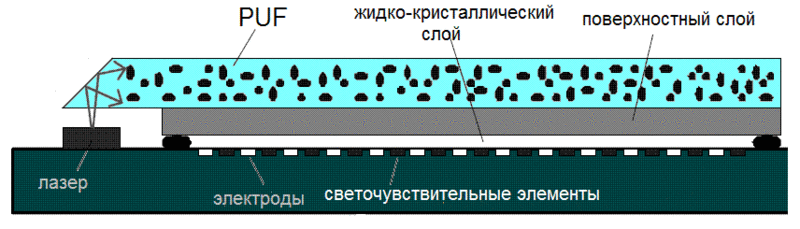
\includegraphics[width=0.7\textwidth]{optical.png}
    \caption{общая структура PUF на оптических элементах}
\end{figure}


\subsubsection{PUF на интегральных микросхемах. }
\label{sub:domain:puf_physical_types:ic}

Аналогично пузырькам в оптической системе, в иных средах тоже можно получить неклонируемость. Рассмотрим среду, и так широко используемую в цифровых устройствах - электрические проводники и диэлектрики.
Любое современное технологичное устройство содержит в себе внушительное количество интегральных микросхем. На них и построены PUF данного типа. Несмотря на то, что микросхемы изготавливаются по одному и тому же технологическому процессу, каждая из них достаточно уникальна для корректной работы PUF. Это может быть использовано в системах информационной безопасности как уникальный идентификационный признак устройства.

Один из вариантов построения такой PUF: интегральная микросхема покрывается слоем защитного вещества со вкраплениями диэлектрика. Эти вкрапления имеют случайные размер и форму. Под этот слой подводятся электроды"=датчики. В совокупности с защитным слоем каждый такой электрод обретает свойства конденсатора случайной (зависящей от вкраплений диэлектрика в защитный слой) ёмкости. Очевидно, что случайность ёмкости каждого конденсатора достигается при размере частиц, сравнимом с размером между электродами.


\subsubsection{PUF на полевых транзисторах. }
\label{sub:domain:puf_physical_types:transistors}

В основе таких PUF лежит особенность полевых транзисторов задерживать сигнал, проходящий по нему на непредсказуемое время, зависящее от физических свойств материала транзистора (именно из"=за материала такие PUF ещё называют кремниевыми). Физическая система PUF будет состоять из набора пар транзисторов и триггеров"=арбитров. Триггер будет давать на выход 0 или 1 в зависимости от того, сигнал с какого из пары транзисторов пришёл к нему раньше. Подавая на вход этому набору некоторый сигнал"=запрос, на выходе исследователь получит набор значений триггеров - реакцию системы на запрос, уникальную для данного устройства, в состав которого включаются упомянутые транзисторы.

Неклонируемость строится на физической неидеальности процесса производства. Изучение функции для последующего математического прогноза реакции на запрос возможно только полным перебором входных сигналов, что является достаточно вычислительно сложной задачей.


\subsubsection{PUF на магнитных элементах. }
\label{sub:domain:puf_physical_types:magnetic}

Практическое применение - уникальный идентификатор магнитной полосы банковской карты. Частицы феррита бария, содержащиеся в пасте"=основе магнитной полосы, также имеют случайный размер и форму. Логично сделать вывод, что на случайности их распределения можно построить PUF. Неклонируемость снова опирается на физическую неидеальность процесса производства. Неточности и погрешности не дадут повторить рисунок частиц феррита бария в  точности. А математическое моделирование не препятствует выполнению данной PUF её задачи.
\begin{figure}[ht]
    \centering
    \label{fig:domain:puf_physical_types:magnetic}
    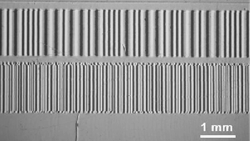
\includegraphics[width=0.55\textwidth]{magneticstripe.png}
    \caption{структура магнитной полосы -- варианта магнитной PUF}
\end{figure}

\subsection{Виды PUF по принципу работы. }
\label{sub:domain:puf_types}


\subsubsection{PUF типа арбитр (Arbiter PUF). }
\label{sub:domain:puf_types:arbiter}

Физически неклонируемые функции по типу арбитра - разновидность физически неклонируемых функций на основе задержек. Идея состоит в том, чтобы привнести состояние гонки между двумя путями микросхемы. Оба пути заканчиваются элементом"=арбитром, который определяет какой из путей был быстрее и выдает соответствующее бинарное значение.
\begin{figure}[ht]
    \centering
    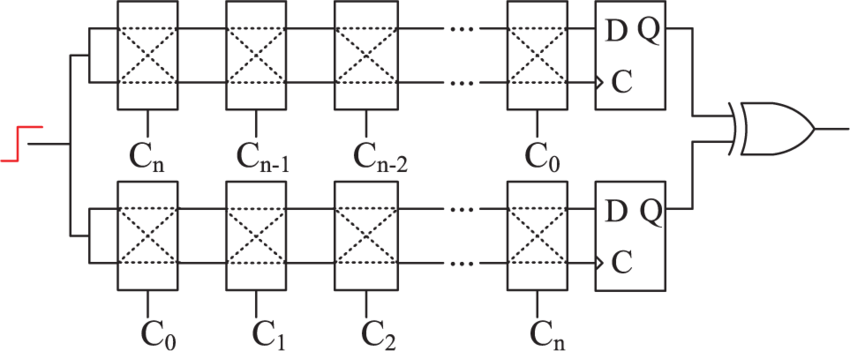
\includegraphics[width=0.7\textwidth]{arbiter.png}
    \caption{PUF типа арбитр}
    \label{fig:domain:puf_types:arbiter}
\end{figure}

Основная идея реализации этого типа PUF состоит в построении двух идентичных путей сигнала на одном кристалле интегральной схемы. Такие пути называются симметричными и имеют очень близкие по значению длины и промежутки времени распространения сигнала. Однако, они не являются полностью идентичными ввиду различных задержек $d$ на каждом отрезке пути, обусловленными вариацией техпроцесса. Измерение различий во времени пути сигнала осуществляется с помощью одновременной подачи сигналов на входы симметричных путей и регистрации моментов получения сигналов на выходах каждого из путей. Симметричные пути проектируются в виде конфигурируемых соеднений на основе мультиплексоров, управляя количеством которых, а также сигналами, подаваемыми на управляющие их входы, можно создавать различные комбинации путей прохождения сигнала. Для сравнения симметричных путей применяется арбитр -- элемент, значение на выходе которого определяется тем, по какому пути сигнал достиг его раньше. Простейший вариант арбитра - синхронный D-триггер. Схема такого построения PUF показана на рисунке~\ref{fig:domain:puf_types:arbiter}.

Таким образом, в качестве битов запроса $C_i \in \{0,1\} $ принимаются сигналы управляющих входов мультиплексоров, а выходным значением $R_i$ будет являться сигнал на выходе элемента-арбитра, к входам которого подключены выходы симметричных путей. Возможна также другая реализация, где вместо мультиплексоров используются трёхстабильные буферы. PUF типа арбитр на трёхстабильных буферах потребляет значительно меньше энергии при меньшей площади кристалла.

\subsubsection{PUF на базе кольцевого генератора (RO"=PUF). }
\label{sub:domain:puf_types:ring_oscillator}

Физически неклонируемые функции на базе кольцевых генераторов также используют неконтролируемые изменения задержек процессов цифровых компонентов в качестве источника случайности. Когда эти компоненты образуют кольцевой генератор, частоты его выходных сигналов различаются, что и используется при формировании бинарного ответа.

\begin{figure}[ht]
    \centering
    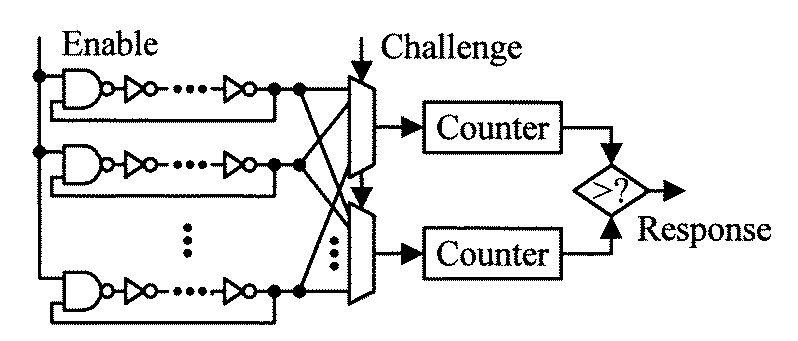
\includegraphics[width=0.8\textwidth]{ro-puf.png}
    \caption{PUF на базе кольцевого генератора}
    \label{fig:domain:puf_types:ring_oscillator}
\end{figure}

Данный тип физически неклонируемой функции основан на использовании частотных характеристик кольцевых генераторов, представляющих собой схемы из подключенных инверторов с отрицательной обратной связью. Число инверторов в цепи должно быть нечётным для обеспечения получения, выходного сигнала в виде меандра, частота которого как раз и определяется задержкой распространения обратного сигнала. Схема кольцевого генератора показана на рисунке~\ref{fig:domain:puf_types:ring_oscillator}.

Для обеспечения стабильного состояния каждый генератор дополнен элементом элементом \emph{И} на входе. Управление ФНФ на основе кольцевого генератора осуществляется путём подачи вектора входных сигналов $C_i$ на управляющие входы мультиплексоров, подсоединённых к выходам кольцевых генераторов. Основой формирования ответа $R_i$ является результат сравнения частот генераторов. Таким образом, набор генераторов будет имет произвольное соотношение частот и уникально характиризовать устройство, в котором они реализованы.

\subsubsection{PUF на базе статического ОЗУ (SRAM PUF). }
\label{sub:domain:puf_types:sram}
Стати
Принцип работы физически неклонируемых функций на базе статического оперативного запоминающего устройства (СОЗУ) основан на случайности состояния части ячеек СОЗУ при включении.

\begin{figure}[ht]
    \centering
    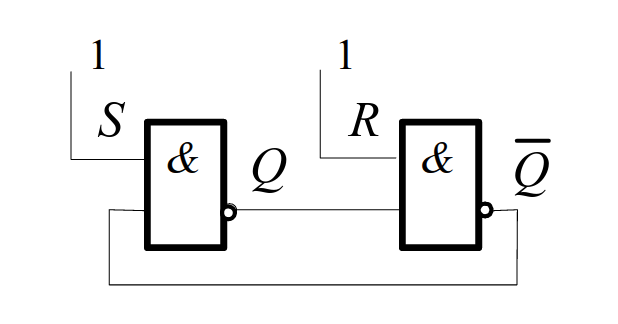
\includegraphics[width=0.76\textwidth]{rs_sram.png}
    \caption{PUF на базе ячейки статического ОЗУ в виде RS-триггера}
    \label{fig:domain:puf_types:sram}
\end{figure}

Статические оперативные запоминающие устройства (СОЗУ) широко используются в вычислительной технике для хранения данных. Непосредственно запоминающий элемент СОЗУ (ячейка) состоит из четырех транзисторов, реализующих два инвертора с перекрестными обратными с связями. Подобная ячейка всегда находится в одном из двух состояний, что, в свою очередь, позволяет использовать ее для хранения одного бита информации. Примером такой ячейки может служить RS-триггер, реализованный на двух логических элементах \emph{2И-НЕ}, представленный на рисунке~\ref{fig:domain:puf_types:sram}. Высокий уровень сигнала (логическая единица), подаваемый одновременно на оба входа RS-триггера, позволяет сохранять предыдущее состояние. При включении питающего напряжения все ячейки СОЗУ устанавливаются в одно из двух возможных состояний -- 0 или 1; причем в силу симметрии RS-триггера априори неизвестно, какое конечное состояние примет ячейка. Экспериментально подтверждено, что большинство ячеек СОЗУ при включении питающего напряжения преимущественно переходят в одно из двух состояний. Причиной этого является несимметричность прямых и обратных связей RS-триггера, обусловленная особенностями технологии изготовления.


\subsubsection{PUF типа <<бабочка>> (Butterfly PUF). }
\label{sub:domain:puf_types:butterfly}
Физически неклонируемые функции по типу бабочки имитирует работу ячейки СОЗУ, формируя перекрестные обратные связи для получения бистабильной схемы. В отличие от ФНФ на базе ячейки СОЗУ, данная функция состоит из двух асинхронных D-триггеров. Схема принудительно переводится в неустойчивое состояние путем подачи взаимоюсключающих сигналов на входы триггеров, после чего схема переходит в одно из двух стабильных состояний, которое зависит от случайной разности задержек в паре линий обратной связи и линии входного сигнала~\cite{yarmolik_vashinko}. Своё название данная разновидность получила благодаря виду схемы, на которой она реализована.
\begin{figure}[ht]
    \centering
    \label{fig:domain:puf_types:butterfly}
    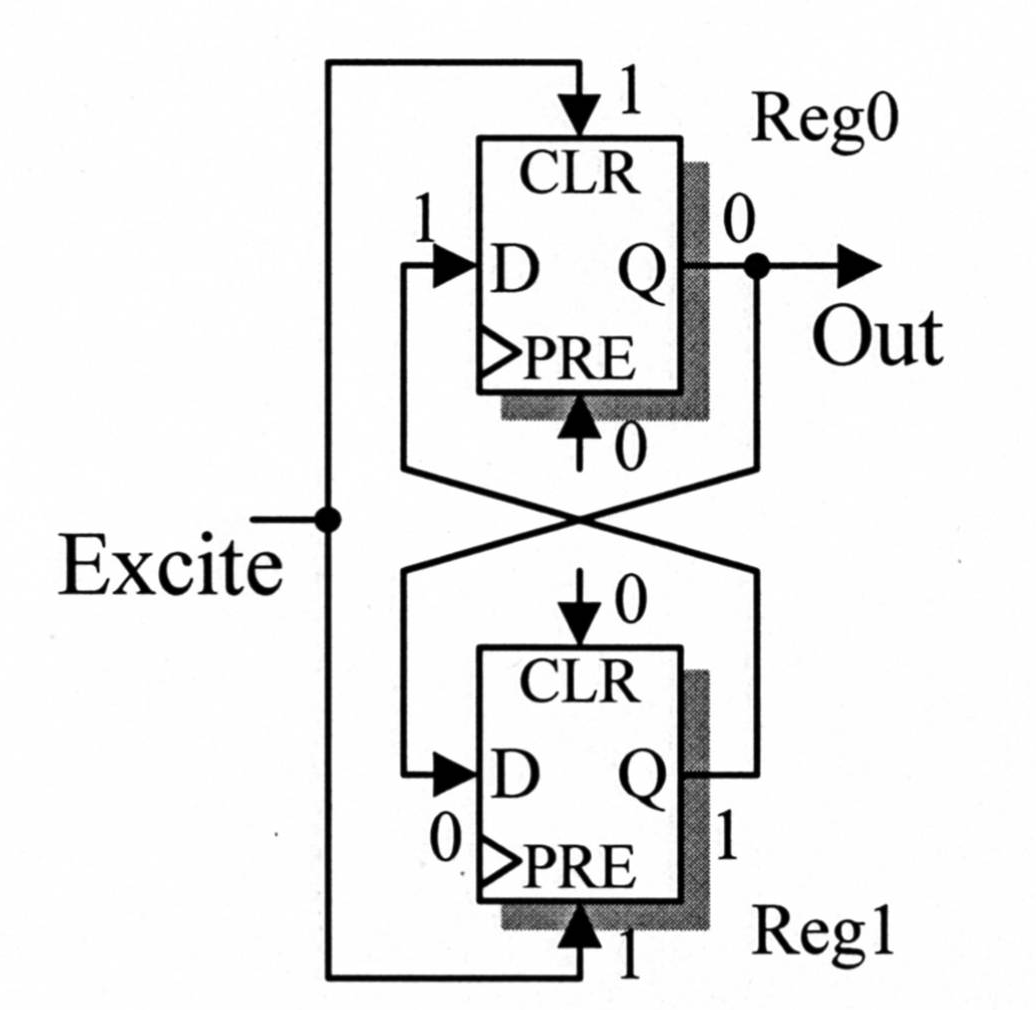
\includegraphics[width=0.6\textwidth]{butterfly.png}
    \caption{PUF типа <<бабочка>>}
\end{figure}


\subsubsection{PUF на основе сбоев (Failure PUF). }
\label{sub:domain:puf_types:failure_puf}

Этот тип физически неклонируемых функций основываются на сбоях в поведении комбинаторных логических схем. В идеале у комбинаторной схемы нет внутреннего состояния, что означает, что стационарный выход полностью определяется его входными сигналами. Однако, когда логическое значение на входе изменяется, для достижения стационарного значения на выходе требуется некоторое время. Появление сбоя определяется различиями в задержках различных логических цепей от входов к выходному сигналу. Так как задержки определенных образцов комбинаторных схем вызваны случайными изменениями процесса, появление, количество и форма сбоев выходных сигналов также будут случайными и характерными для определенных образцов схемы. Поэтому оценка поведения сбоев таких схем может быть использована для ответа физически неклонируемой функции.

Стоит заметить, что в данном списке перечислены лишь базовые варианты реализации PUF. На их основе и на основе комбинаций этих типов может быть построено огромное множество различных сложных PUF~\cite{cryptowiki_pufs, rmaes_pufs}.


\subsection{Использование PUF для идентификации и аутентификации цифровых устройств}
\label{sub:domain:puf_auth}
Аутентификация традиционно характеризуется как процесс проверки того, что сущность владеет конкретной информацией, например, паролем, обладает конкретными свойствами, или же является именно тем, за что себя выдает. Многофакторная аутентификация представляет собой комбинацию этих проверок. Аутентификация на основе физически неклонируемых функций подразумевает наличие разных независимых устройств, каждое из которых характеризуется набором паролей (т.е. в данном случае -- набором пар запрос"=ответ), который однозначно идентифицирует эти устройства, то есть, в какой-то степени, аутентификацию на основе PUF можно считать многофакторным механизмом.

Множество возможных применений ФНФ также включает шифрование информации, обнаружение вредоносных изменений структуры интегральной микросхемы, контроль специфических функций устройств и многие другие. Каждый из сценариев использования предъявляет определенные требования к свойствам используемой ФНФ. В частности, для использования в криптографических целях, ФНФ должна быть устойчива к атакам моделирования, т.е. должна препятствовать построению более-менее точной модели своей структуры и/или поведения. Это же применимо и к протоколам аутентификации на основе ФНФ. Общее правило -- чем больше контроля над своими входными и выходными параметрами ФНФ предоставляет приложению, тем лучше оно должно быть защищено от таких атак.

Применительно к аутентификации на основе ФНФ применяют термины \emph{электронный ключ (токен)} -- для обозначения утройства, оснащённого ФНФ, чья подлинность проверяется, например, смарт-карта или RFID-метка~\cite{rfid_puf}, и \emph{доверенный сервер} -- для обозначения стороны, располагающей истинными данными идентификации конкретных устройств.

Существует два основных подхода к осуществлению системы аутентификации, основанной на физически неклонируемых функциях. Первый подход состоит в получении стойкого и безопасного криптографического ключа из ответа физически неклонируемой функции и использовании этого ключа в каком"=либо из протоколов аутентификации. В этом случае ФНФ используется в качестве или как составная часть генератора истинно случайных чисел с показателями, достаточными для его применения в криптографических целях. Секретность ключа повышается тем, что в открытом виде могут храниться только данные, использованые для его генерации, в данном случае -- наборы пар $\crp$. Следовательно, воспроизвести ключ возможно только при использовании исходной ФНФ и с данным набором входных данных. Для этого подхода достаточно довольно простой ФНФ (т.н. \emph{weak PUF, слабая ФНФ}), способной сгенерировать достаточное для построения ключа количество случайной информации, но при этом устройство должно содержать реализацию криптографического алгоритма, чтобы из входного набора сконструировать ключ. К сожалению, этот метод уязвим к атаке по стороннему каналу (\emph{side-channel attack}): злоумышленник может получить секретный ключ, используя уязвимости в аппаратной реализации алгоритма~\cite{pufbased_auth,puf_cryptography}.

Другой подход состоит в разработке схемы аутентификации, которая напрямую применяет уникальность и непредсказуемость поведения пары запроса"=ответа отдельного объекта. Такая схема состоит из двух фаз (регистрации в системе и подтверждения подлинности).

В первой фазе, каждый объект проходит регистрацию у проверяющего. Во время этой фазы проверяющий записывает идентификатор каждого объекта и собирает значительное подмножество пар запрос"=ответ каждого объекта (устройства) для случайно сгенерированных запросов. Собранные пары запрос"=ответ хранятся в базе данных проверяющего.

Во время фазы подтверждения, объект (устройство) посылает проверяющему свой идентификатор. Проверяющий находит его в базе данных, выбирает оттуда случайную пару запрос"=ответ, которая соответствует полученному идентификатору. Запрос посылается объекту, объект вычисляет физически неклонируемую функцию и посылает ответ. Проверяющий сравнивает этот ответ со значением из базы данных, и если проверка прошла успешно, тообъект аутентифицирован, иначе -- аутентификация отклонена. Использованная пара запрос"=ответ удаляется из базы данных для исключения возможности сохранения результатов третьей стороной. Корректность данной схемы аутентификации обеспечивается тем фактом, что ответы физически неклонируемых функций воспроизводимы самим объектом в течение долгого времени.
Однако, подход в описанном выше виде имеет существенные минусы:
\begin{itemize}
  \item Число возможных пар $ \crp $ может быть, а в реальных PUF почти всегда является очень большим. Вследствие этого, регистрация устройства путем сбора достаточного для последуещей аутентификации количества пар не всегда возможно за приемлемое время.
  \item Несмотря на то, что ответы физически неклонируемых функций воспроизводимы самим объектом, ФНФ редко являются полностью стабильными. Подавляющее большинство реализаций имеют дополнительную зависимость выходного сигнала от побочных эффектов, таких как физический износ устройства, температура окружающей среды, влажность и других параметров. В связи с этим, однозначное соответствие нескольких выходных сигналов $ R $, вызванных одним набором $ C $, не может быть гарантировано.
\end{itemize}

Из-за этих нюансов, использование <<наивной>> реализации протокола не представляет особой практической ценности. Поэтому данный дипломный проект ставит целью исследование и реализацию усовершенствованного протокола аутентификации, учитывающего указанные особенности и предоставлящего достаточный уровень секретности и защиты от перехвата данных или управления третьей стороной.


\subsection{Обзор существующих аналогов}
Подавляющее большинство средств защиты интеллектуальной собственности применительно к цифровым устройствам, в частности, программные средства аутентификации устройств на основе физически неклонируемых функций, а также особенности их реализации сами по себе являются коммерческой тайной. В связи с этим, даже поверхностный анализ и сравнение существующих аналогов не представляется возможным. Однако, целесообразным представляется создание доступного открытого аналога средства аутентификации, которое, в противовес проприетарным решениям компаний"=производителей, могло бы служить удобной базой для дальнейшей развития и затачивания под конкретные нужды энтузиастами разработки цифровых устройств, а также в образовательных целях.


\subsection{Постановка задачи}
В результате выполнения дипломного проекта должно быть разработано программное средство аутентификации цифровых устройств, реализующее протокол взаимодействия между сервером аутентификации и цифровым устройством, включающим в себя некоторую реализацию PUF для однозначной его идентификации. К разрабатываемому программному средству предъявляются следующие требования:
\begin{itemize}
\item разрабатываемое ПО должно работать на операционных системах Linux и Windows;
\item программное средство должно быть выполнено в виде клиент"=серверного приложения;
\item программное средство должно поддерживать работу как в режиме регистрации устройства в базе данных, так и в режиме его аутентификации;
\item принцип работы разрабатываемого ПО не должен быть привязан к конкретному типу аутентифицируемого устройства.
\end{itemize}
 %

% Глава 2 Используемые технологии
\section{Используемые технологии}
\label{sec:techs:intro}

Выбор технологий является важным предварительным этапом разработки сложных информационных систем.
Платформа и язык программирования, на котором будет реализована система, заслуживает большого внимания, так как исследования показали, что выбор языка программирования влияет на производительность труда программистов и качество создаваемого ими кода~\cite[c.~59]{mcconnell_2005}.

Ниже перечислены некоторые факторы, повлиявшие на выбор технологий:
\begin{itemize}
\item Разрабатываемое ПО должно работать на операционных системах Linux и Windows.
\item Программное средство должно быть выполнено в виде клиент-серверного приложения.
\item Дальнейшей поддержкой проекта, возможно, будут заниматься разработчики, не принимавшие участие в выпуске первой версии.
\item Имеющийся разработчик имеет опыт работы с объектно"=ориентированными и с функциональными языками программирования.
\end{itemize}

Основываясь на приведенных факторах, целесообразно выбрать в качестве платформы разработки язык Python. Приняв во внимание необходимость обеспечения доступности дальнейшей поддержки ПО, возможно, другой командой программистов, целесообразно не использовать малоизвестные и сложные языки программирования.

Для реализации поставленной задачи существует необходимость в написании серверного приложения. Эту задачу можно облегчить путём использования набора прикладных библотек (фреймворка) Flask, предназначенного для быстрого прототипирования и реализации веб-приложений различной степени сложности.

Далее проводится характеристика используемых технологий и языков программирования более подробно.



\subsection{Язык программирования Python}
\label{sub:techs:python}
Python — высокоуровневый язык программирования общего назначения, ориентированный на повышение производительности разработчика и читаемости кода. Синтаксис ядра Python минималистичен. В то же время стандартная библиотека включает большой объём полезных функций.

Python поддерживает несколько парадигм программирования, в том числе структурное, объектно-ориентированное, функциональное, императивное и аспектно-ориентированное. Основные архитектурные черты — динамическая типизация, автоматическое управление памятью, полная интроспекция, механизм обработки исключений, поддержка многопоточных вычислений и удобные высокоуровневые структуры данных. Код в Python организовывается в функции и классы, которые могут объединяться в модули (они в свою очередь могут быть объединены в пакеты).

Эталонной реализацией Python является интерпретатор CPython, поддерживающий большинство активно используемых платформ. Он распространяется под свободной лицензией Python Software Foundation License, позволяющей использовать его без ограничений в любых приложениях, включая проприетарные. Есть реализации интерпретаторов для JVM (с возможностью компиляции), MSIL (с возможностью компиляции), LLVM и других. Проект PyPy предлагает реализацию Python на самом Python, что уменьшает затраты на изменения языка и постановку экспериментов над новыми возможностями.

Python — активно развивающийся язык программирования, новые версии (с добавлением/изменением языковых свойств) выходят примерно раз в два с половиной года. Вследствие этого и некоторых других причин на Python отсутствуют стандарт ANSI, ISO или другие официальные стандарты, их роль выполняет CPython.

Отличительные особенности языка Python:
\begin{itemize}
  \item Простой. Python – простой и минималистичный язык. Чтение хорошей программы на Python очень напоминает чтение английского текста. Такая псевдо-кодовая природа Python является одной из его самых сильных сторон. Она позволяет сосредоточиться на решении задачи, а не на самом языке.
  \item Свободный и открытый. Python – это пример свободного и открытого программного обеспечения – FLOSS (Free/Libré and Open Source Software). Пользователь имеет право свободно распространять копии этого программного обеспечения, читать его исходные тексты, вносить изменения, а также использовать его части в своих программах. В основе свободного ПО лежит идея сообщества, которое делится своими знаниями. Это одна из причин, по которым Python так хорош: он был создан и постоянно улучшается сообществом, которое хочет сделать его лучше.
  \item Язык высокого уровня. При написании программы на Python разработчику не нужно отвлекаться на такие низкоуровневые детали, как управление памятью и т.п.
  \item Портируемый. Благодаря своей открытой природе, Python был портирован на множество платформ. Программы на Python могут запускаться на любой из этих платформ без каких-либо изменений (если программа не использует системно-зависимые функции). Python можно использовать в GNU/Linux, Windows, FreeBSD, Macintosh, Solaris, OS/2, Amiga, AROS, AS/400, BeOS, OS/390, z/OS, Palm OS, QNX, VMS, Psion, Acorn RISC OS, VxWorks, PlayStation, Sharp Zaurus, Windows CE и множестве других платформ.
  \item Интерпретируемый. Python не требует компиляции в бинарный код. Программа выполняется из исходного текста. Python сам преобразует этот исходный текст в некоторую промежуточную форму, называемую байткодом, а затем переводит его на машинный язык и запускает. Всё это заметно облегчает использование Python, поскольку нет необходимости заботиться о компиляции программы, подключении и загрузке нужных библиотек и т.д. Вместе с тем, это делает программы на Python намного более переносимыми.
  \item Объектно-ориентированный. Python поддерживает как процедурно-ориентированное, так и объектно-ориентированное программирование. Python предоставляет простые, но мощные средства для ООП, особенно в сравнении с такими большими языками программирования, как C++ или Java.
  \item Расширяемый. Если необходимо добиться очень высокой производительности некоторой части программы или использовать некоторые другие возможности более низкоуровневых языков, можно разработать эту часть программы на C или C++, а затем вызывать её из программы на Python.
  \item Встраиваемый. Python можно встраивать в программы на C/C++, чтобы предоставлять возможности написания сценариев их пользователям.
  \item Обширные библиотеки. Стандартная библиотека Python просто огромна. Она может помочь в решении самыхразнообразных задач, связанных с использованием регулярных выражений, генериро-ванием документации, проверкой блоков кода, распараллеливанием процессов, база-ми данных, веб-браузерами, CGI, FTP, электронной почтой, XML, XML-RPC, HTML, WAV файлами, криптографией, GUI и другими системно-зависимыми вещами. Всё это доступно абсолютно везде, где установлен Python. В этом заключается философия Python <<Всё включено>>.Кроме стандартной библиотеки, существует множество других высококачественных биб-лиотек, доступных в каталоге пакетов.
\end{itemize}

\subsubsection{Объектно-ориентированное программирование}
Дизайн языка Python построен вокруг объектно-ориентированной модели программирования. Реализация ООП в Python является элегантной, мощной и хорошо продуманной, но вместе с тем достаточно специфической по сравнению с другими объектно-ориентированными языками. Особенности~\cite{wiki_python, byte_of_python}:
\begin{itemize}
\item Классы являются одновременно объектами со всеми ниже приведёнными возможностями.
\item Наследование, в том числе множественное.
\item Полиморфизм (все функции виртуальные).
\item Инкапсуляция (два уровня — общедоступные и скрытые методы и поля). Особенность — скрытые члены доступны для использования и помечены как скрытые лишь особыми именами.
\item Специальные методы, управляющие жизненным циклом объекта: конструкторы, деструкторы, распределители памяти.
\item Перегрузка операторов (всех, кроме is, '.', '=' и символьных логических).
\item Свойства (имитация поля с помощью функций).
\item Управление доступом к полям (эмуляция полей и методов, частичный доступ, и т. п.).
\item Методы для управления наиболее распространёнными операциями (истинностное значение, len(), глубокое копирование, сериализация, итерация по объекту, …)
\item Метапрограммирование (управление созданием классов, триггеры на создание классов, и др.)
\item Классовые и статические методы, классовые поля.
\end{itemize}

\subsubsection{Функциональное программирование}
Python поддерживает парадигму функционального программирования, в частности:
\begin{itemize}
\item Функция является объектом;
\item Функции высших порядков;
\item Рекурсия;
\item Развитая обработка списков (списочные выражения, операции над последовательностями, итераторы);
\item Аналог замыканий;
\item Частичное применение функции;
\end{itemize}

\subsubsection{Интроспекция}
Python поддерживает полную интроспекцию времени исполнения. Это означает, что для любого объекта можно получить всю информацию о его внутренней структуре.
Применение интроспекции является важной частью того, что называют pythonic style, и широко применяется в библиотеках и фреймворках Python, таких как PyRO, PLY, Cherry, Django и др., значительно экономя время использующего их программиста.

\subsubsection{Итераторы и генераторы}
В программах на Python широко используются итераторы. Цикл for может работать как с последовательностью, так и с итератором. Все коллекции, как правило, предоставляют итератор. Объекты определённого пользователем класса тоже могут быть итераторами. Подробнее об итераторах можно узнать в разделе о функциональном программировании. Модуль itertools стандартной библиотеки содержит много полезных функций для работы с итераторами.

Другой интересной возможностей языка являются генераторы — функции, сохраняющие внутреннее состояние: значения локальных переменных и текущую инструкцию. Генераторы могут использоваться как итераторы для структур данных и для ленивых вычислений.
При вызове генератора функция немедленно возвращает объект-итератор, который хранит текущую точку исполнения и состояние локальных переменных функции. При запросе следующего значения (посредством метода next(), неявно вызываемого в цикле for) генератор продолжает исполнение функции от предыдущей точки останова до следующего оператора yield или return.


\subsection{Sandia National Laboratories PUF Analysis Tool (SPAT)}
\label{sec:techs:spat}
Sandia National Laboratories PUF Analysis Tool - программное средство с открытым исходным кодом, созданное Sandia Corporation для симуляции физически неклонируемых функций, наглядной демонстрации и оценки их статистических свойств. Этот инструмент был создан главным образом для использования в образовательных целях.

Функции данной программы не ограничиваются только лишь симуляцией, она с равным успехом может анализировать статистические свойства реальных физических PUF.
Программа представляет собой набор следующих модулей:
\begin{itemize}
  \item модуль взаимодействия с физическими устройствами;
  \item модуль симуляции PUF (может быть расширен пользователем);
  \item модуль анализа свойств PUF независимо от реализации (физическая или симуляция).
  \item графический интерфейс
\end{itemize}
SPAT может быть использована для визуализации:
\begin{itemize}
  \item влияния шума на выходной сигнал PUF;
  \item метрик среднего значени шума в микросхеме;
  \item динамики расстояния Хэмминга выходного сигнала в зависимости от динамики входного.
  \item свойств случайности для данного чипа, таких как энтропия.
\end{itemize}
\begin{figure}[ht]
    \centering
    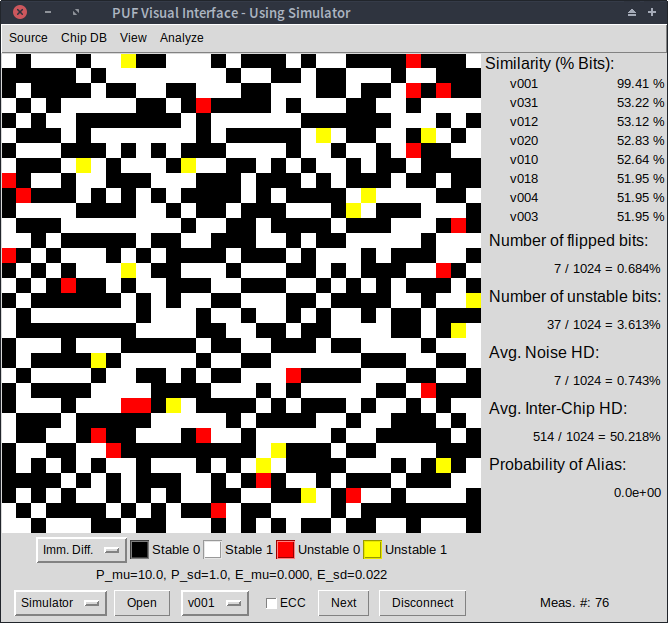
\includegraphics[width=0.7\textwidth]{spat.png}
    \caption{Окно программы SPAT с результатами статистического анализа виртуальной RO-PUF}
    \label{fig:techs:spat}
\end{figure}
 %

% Глава 3 Проектирование архитектуры программного средства
\section{Архитектура и модули системы}

Разработанное программное обеспечение является сложным программным комплексом, состоящим из различных модулей:
\begin{itemize}
    \item модуль построения компактной модели PUF;
    \item модуль симуляции PUF;
    \item модуль контроля доступа;
    \item модуль проверки подлинности.
\end{itemize}

Вышеописанные модули опираются на следующие группы классов, разработанные в рамках дипломного проекта:
\begin{itemize}
    \item Библиотека протокола аутентификации. Написана на языке Python. Содержит методы для проведения основных операций, используемых в проктоколе аутентификации.
    \item Библиотека машинного обучения (для построения модели PUF). Написана на языке программирования Haskell и содержит реализацию алгоритма наивного байесовского классификатора (Naive Bayes Classifier), о котором будет рассказано далее.
    \item Набор классов для работы с PUF. Написана на языке Python. Содержит классы для манипуляции с объектами типа Challenge и Response, которые построены на базе битового массива (bitarray). Реализует реализации алгоритмов генерации, сравнения, сложения и других операций над битовыми массивами, необходимых для обработки сингалов PUF.
    \item Слой взаимодействия с устройствами на языке Python. Является легковесным контрактом, предоставляющим единый интерфейс обращения к подключенным устройствам.
\end{itemize}

Общий принцип взаимодействия компонентов и пример сценария использования программной системы приведен на рисунке~\ref{fig:architecture:flow}. В следующих подразделах более подробно описано назначение и устройство каждого из логических модулей ПС.

\afterpage{
  \begin{landscape}
  \thispagestyle{lscape}
  \begin{figure}[t!]
  \centering
    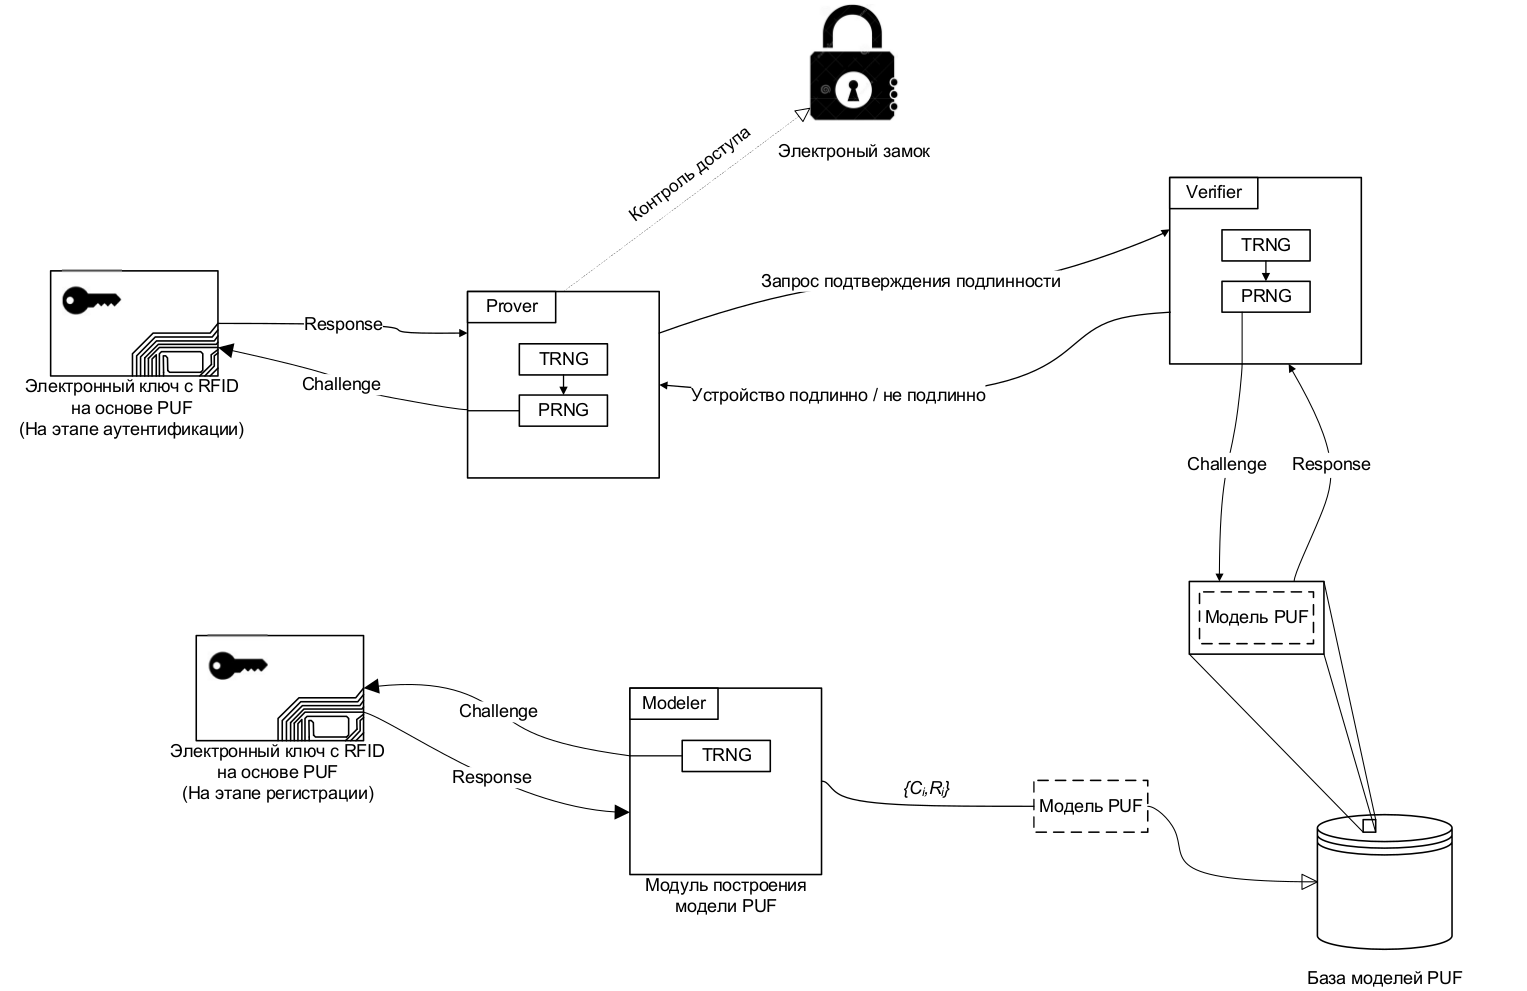
\includegraphics[scale=0.40]{flow.png}
    \caption{ Схема работы программной системы }
    \label{fig:architecture:flow}
  \end{figure}
  \end{landscape}
}


\subsection{Модуль построения компактной модели PUF}
Главная особенность реализуемого протокола аутентификации -- использование компактной модели PUF в качестве эталонного показателя подлинности. Поэтому, закономерно рассмотреть особенности построения этой модели.

Для построения компактной модели ФНФ был выбран наивный байесовский классификатор -- широко используемый метод машинного обучения~\cite{manning_ir}, который при своей относительной простоте реализации, позволяет добиться очень неплохих результатов классификации. На выбор повлияло также то, что задача обучения модели ФНФ сводится к задаче классификации множества входных битовых строк $C$ на выходные классы -- <<0>> и <<1>>.

Наивный баейсовский классификатор – семейство простых вероятностных классфикаторов, которые основываются на теореме Байеса. Классификатор использует решающее правило MAP (maximum a posteriori), которое ставит в соответствие объекту наиболее вероятную для него метку и описывается формулой~\cite{mitchell_ml}:
\begin{equation}
  \label{eq:architecture:bayes}
  y = \underset{c\,\in\,C}{argmax}~P(C) \prod\limits_{i=1}^{n} P(x_i|C)
\end{equation}
\begin{explanation}
где & $ P(C) $ & априорная вероятность принадлежности объекта к классу $C$; \\
    & $ P(x_i|C) $ & правдоподобие принадлежности объекта к классу $C$, исходя из значения аттрибута
$x_i$; \\
    & $ x_i $ & атрибут объекта.
\end{explanation}

При работе с непрерывными аттрибутами используется предположение, что аттрибуты выбираются из независимых непрерывных нормальных распределений. Таким образом, задача обучения классификатора заключается в нахождении параметров распределения -- математического ожидания и дисперсии -- для каждого из аттрибутов, что позволит вычислять $P(x_i|C)$.

Известно, что величины случайных отклонений, связанные с вариацией технологического процесса, подчняются нормальному распределению. Поэтому вполне очевидным является использование байесовского классификатора на основе нормального закона распределения:
\begin{equation}
  \label{eq:architecture:gaussian_bayes}
  P(x_i = \nu|C) = \frac{1}{\sqrt{2 \pi {\sigma}_{ic}^2}} \, exp(-\frac{\nu - \overline{x_{ic}}^2}{2\sigma_{ic}^2})
\end{equation}
\begin{explanation}
где & $x_{ic}$ & среднее значение атрибута, рассчитанное для объектов, принадлежащих
классу $C$; \\
    & $ \sigma_{ic}^2 $ & выборочная дисперсия значания атрибута объектов из класс $C$.
\end{explanation}

Выборочная дисперсия значения атрибута определяется формулой:
\begin{equation}
  \label{eq:architecture:dispersion}
  \sigma_{ic}^2 = \frac{1}{n - 1} \sum\limits_{x \in C} (x_i - \overline{x_{ic}}^2)
\end{equation}

В нашем случае, когда классифицируемыми объектами являются битовые массивы, удобно представить их виде векторов $s$ значених их битов: $s_i \in \{0, 1\}$. Тогда каждый бит массива будет являться атрибутом классифицируемого объекта. В дополнение к этому, благодаря ограниченному набору значений атрибутов ($\{0, 1\}$), вычисления можно значительно оптимизировать.

Модуль построения компактной модели PUF реализован на языке Haskell. На рисунке TODO представлена схема алгоритма классификатора. Листинги \ref{lst:architecture:naive_bayes_hs} и \ref{lst:architecture:statistics_hs} содержит фрагменты кода программного модуля, непосредственно относящиеся к решению задачи классификации. Модуль классификатора поддерживает работу в параллельном режиме на многопроцессорных устройствах, что значительно сокращает время обучения модели.


\lstinputlisting[
    style=commonstyle,
    caption={Наивный байесовский классификатор},
    label=lst:architecture:naive_bayes_hs
]{src/NaiveBayes.hs}

\lstinputlisting[
    style=commonstyle,
    caption={Статистические функции, используемые в классификаторе},
    label=lst:architecture:statistics_hs
]{src/Statistics.hs}

\begin{figure}[!h]
    \centering
    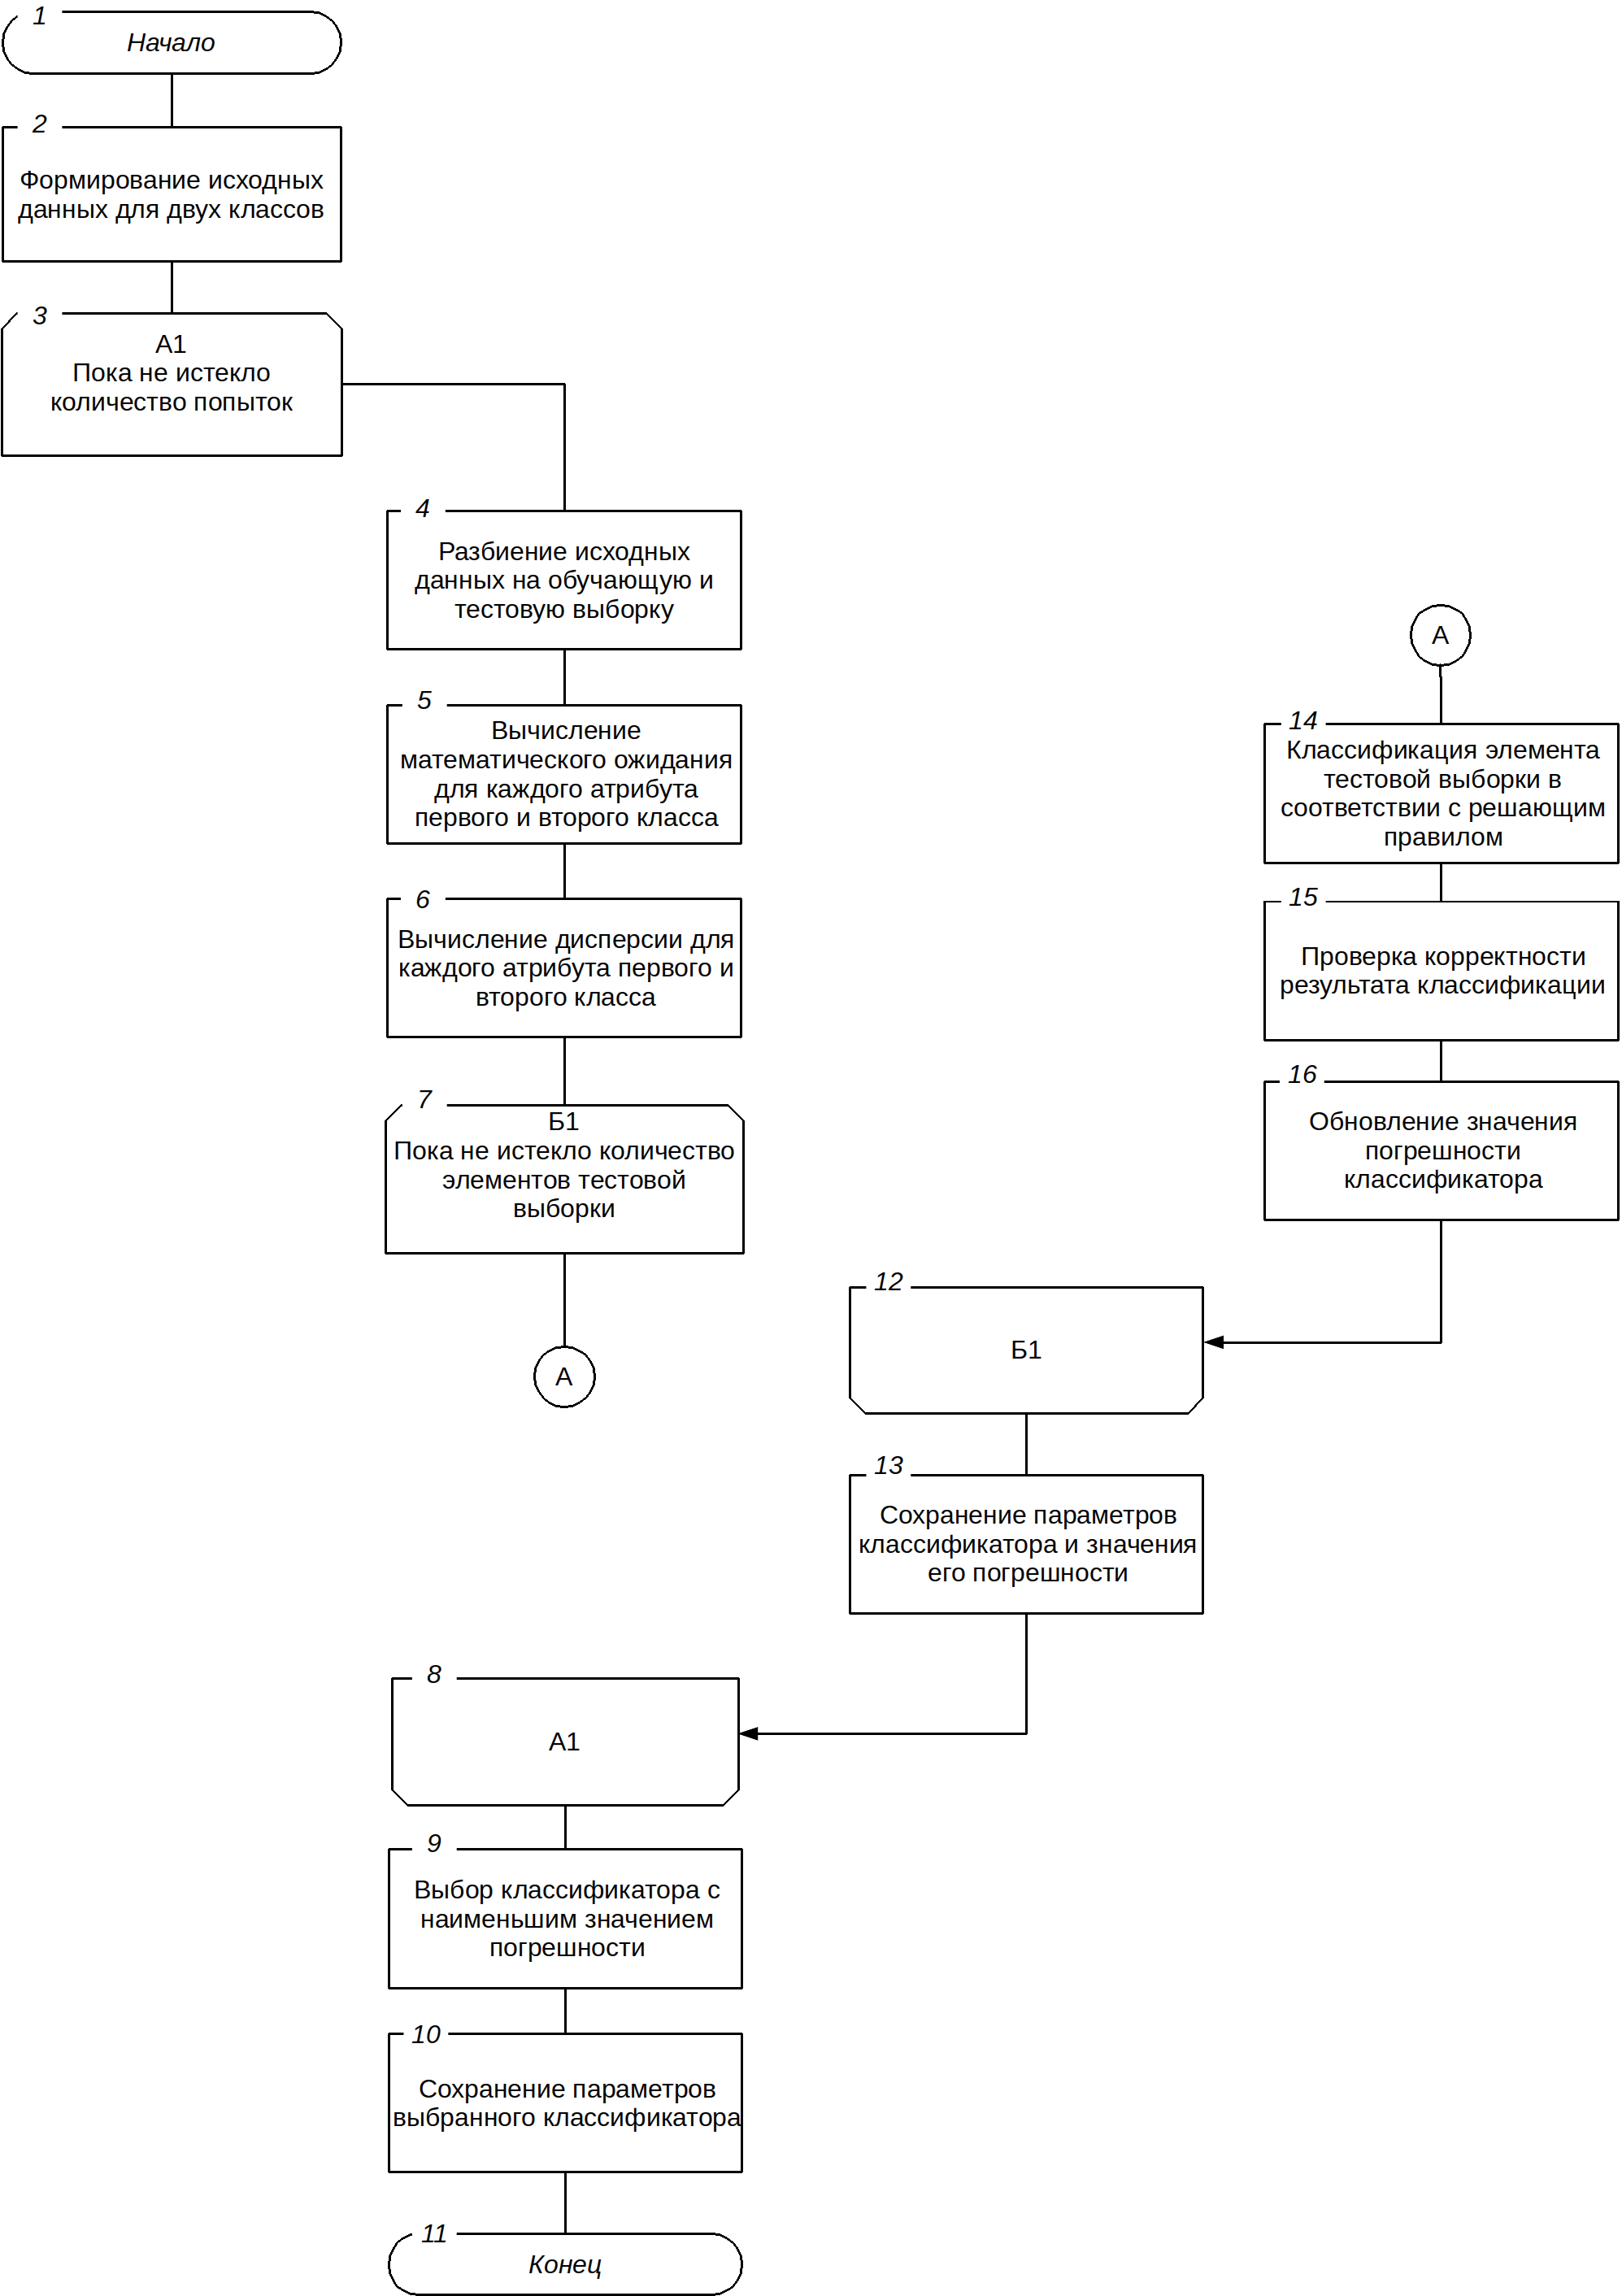
\includegraphics[width=0.95\textwidth]{bayes.png}
    \caption{Схема алгоритма обучения модели методом наивного байесовского классификатора}
    \label{fig:architecture:bayes}
\end{figure}

\subsection{Модуль симуляции PUF}
В целях упрощения разработки, тестирования и демонстрации функциональности ПС было принято решение использовать программную симуляцию физически неклонируемой функции вместо аппаратной реализации. Более того, симуляция PUF может применяться также и конечным пользователем, к примеру, для моделирования PUF со статистическими параметрами, приближенными к таковым у реальной PUF и определения оптимальных параметров функционирования протокола. Таким образом, симуляция PUF из удобного инструмента на этапе разработки переросла в одну из функций программного средства.

Принцип генераций случайных величин, которые будут использованы в качестве физических параметров виртуальной PUF, основан на том факте, что естественные отклонения физических параметров транзисторов (длина, ширина, толщина оксидной плёнки) от заданных значений на этапе их изготовления моделируются распределением, близким к нормальному, так как являются следствиями недетерминированных физических процессов~\cite{gauss_wiki,process_variation}.

\begin{figure}[!h]
    \centering
    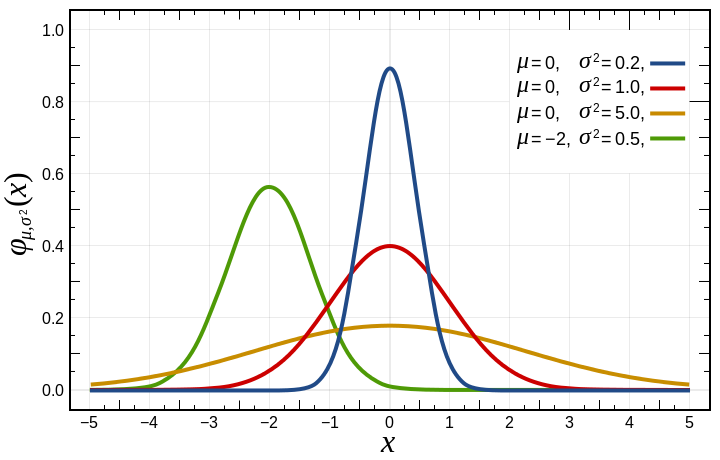
\includegraphics[width=0.85\textwidth]{gauss.png}
    \caption{График функции плотности вероятности для нормального распределения}
    \label{fig:architecture:normal_pd}
\end{figure}

При симуляции физически неклонируемой функции важно учитывать некоторые статистические характеристики, обусловленные нормальным законом распределения значений величин отклонений физических параметров. В частности, из данного факта следует следующее:
\begin{itemize}
  \item Вероятность получения на выходе единицы равна вероятности получения на выходе нуля для всего множества векторов входных сигналов, т.е. $P(r = 0) = P(r = 1) = 0,5 $. Следовательно, в идеальном случае ровно половина возможных векторов входных сигналов соответствует единице на выходе, и ровно половина -- нулю.
  \item Ответы на похожие запросы имеют большую вероятность совпадения. Под похожими понимаются запросы с минимальным расстояниями между ними, рассчитанным по формуле Хэмминга. Иными словами, вероятность того, что ответы $r_0$ и $r_1$ на запросы $C_0$ и $C_1$ будут иметь разные значения, является монотонно возрастающей функцией от расстояния Хэмминга между запросами, т.е. $P(r_0 \neq r_1) = f(HD(C_0, C_1))$. На рисунке ФФФ показана данная зависимость на основании экспериментальных данных.
\end{itemize}

\begin{figure}[!h]
    \centering
    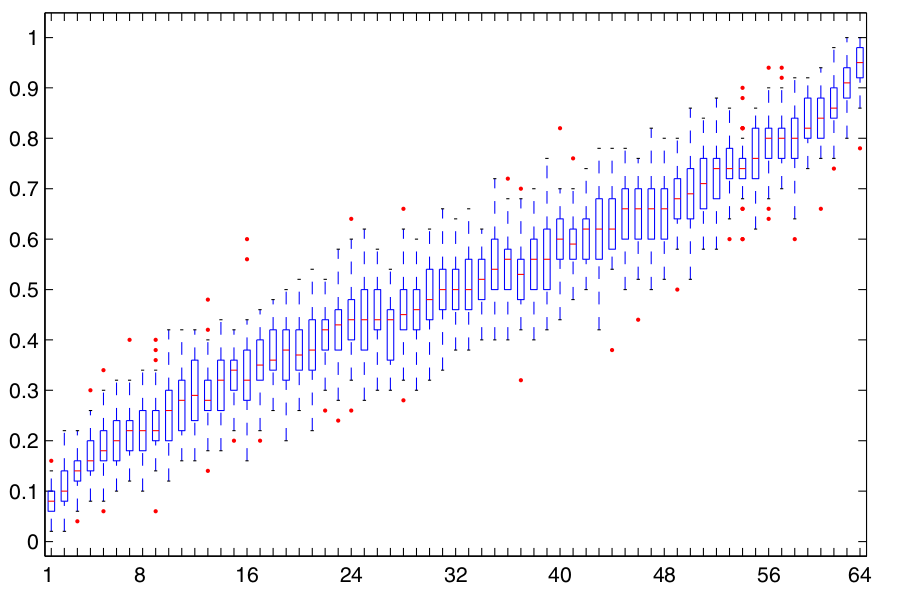
\includegraphics[width=0.75\textwidth]{avalanche.png}
    \caption{График влияния различия входных сигналов на вероятность различия выходных}
    \label{fig:architecture:avalanche}
\end{figure}

При идеальном распределении величин отклонений по нормальному закону выполняется строгий лавинный критерий~\cite{rfid0_puf}, который гласит, что при изменении одного бита аргумента функции выходной бит меняет значение на противоположное с вероятностью 1/2.

Не стоит также забывать, что случайная природа ФНФ не ограничивается лишь вариациями процесса изготовления устройства. Свою случайную компоненту также вносит так называемый <<шум>> -- физические условия окружающей среды, влияющие на параметры полупроводникового устройства. Наиболее остро ощущается влияние высоких температур, при которых функционирует устройство.

Таким образом, для симуляции PUF необходимо учитывать задержки распространения сигналов, привнесенные на этапе производства, а также влияния внешней среды, корректирующие значения этих параметров во время функционирования устройства. Код, используемый для симуляции PUF в программном средстве, учитывает оба эти компонента.

\lstinputlisting[
    style=commonstyle,
    caption={Функиции, используемые для симуляции ФНФ},
    label=lst:architecture:puf_sim
]{src/ropuf.py}


\subsection{Слой взаимодействия с устройствами}
Данная часть программного средства представляет собой абстракцию над любыми типами устройств с PUF (как аппаратными, так и программно симулированными) и предоставляет единый интерфейс взаимодействия с ними. Таким образом, благодаря этому слою, все части программного средства могут единообразно обращаться к любому подключённому устройству с целью регистрации или аутентификации вне зависимости от реализации этого устройства. Для эффективного взаимодействия в рамках этих целей достаточно лишь иметь доступ к собственно функции PUF для обмена сигналами и к некоторым её свойствам, в частности -- ожидаемой длине входного сигнала. С точки зрения программного кода этот слой реализован в виде абстрактного класса device.Device, исходный код которого представлен в листинге \ref{lst:architecture:device}.

\lstinputlisting[
    style=commonstyle,
    caption={Слой взаимодействия с устройствами, класс Device},
    label=lst:architecture:device
]{src/device.py}

В текущей поставке программной системы реализован класс SoftwareArbiter, который представляет собой обертку над программно-симулированным устройством с PUF типа арбитр. Объект класса SoftwareArbiter инициализируется заранее рассчитанными значениями задержек на узлах PUF. Для использования SoftwareArbiter, как и любого другого класса, реализующего методы Device, достаточно вызвать метод объекта SoftwareArbiter.f с битовым массивом значений управляющих сигналов в качестве аргумента. Применительно к PUF типа арбитр функция f рассчитывает выходной бит по следующей формуле:

\begin{equation}
  \label{eq:architecture:arbiter}
  \sum_{j=1}^{N}(-1)^{\rho_j}\delta_j + \delta_{N+1}\mathop{\lessgtr}_{r=1}^{r=0} 0\text{\,,}
\end{equation}
\begin{explanation}
где & $ \rho_j $ & количество единичных битов входного сигнала; \\
    & $ N $ & количество звеньев в цепи; \\
    & $ \delta_j $ & значение задержки на каждом звене. \\
\end{explanation}



\subsection{Библиотека протокола аутентификации}
Реализация протокола аутентификации, используемая в разработанном ПО, является частным случаем т.н. протоколов аутентификации на основе поиска подстроки (substring matching-based authentication protocol). Данный тип протоколов представил в 2012 году M. Majzoobi под названием \emph{Slender  PUF  protocol}~\cite{slender_puf}.

Протокол предназначен для использования со стойкими физически неклонируемыми функциями (Strong PUFs), является очень легковесным и отлично подходит для реализации в устройствах и системах с ограниченными вычислительными ресурсами. В отличие от уже устоявшейся парадигмы, данный протокол не подразумевает раскрытие полной последовательности выходных сигналов, даже в зашифрованном или трансформированном каким-либо другим способом виде. Вместо этого, из последовательности выделяются случайные части и отсылаются как доказательство подлинности. Для аутентификации устройства проверяющая сторона использует заранее сгенерированные шаблоны выходной последовательности (response patterns).

При корректной реализации протокол может обеспечить превосходную устойчивость против любых известных атак, использующих построение модели PUF-устройства с помошью методов машинного обучения. В дополнение к этому, в протокол сразу заложена коррекция ошибок, которые могут возникнуть при получении выходной строки по уже рассмотренным причинам. Благодаря этому, не требуется реализация сторонних алгоритмов коррекции ошибок, отнимающих драгоценные ресурсы, как не требуется и реализация хэш-функций, нечетких экстракторов (fuzzy extractors), предложенных в ранее известных протоколах аутентификации на основе ФНФ.

В основе протокола лежит построение компактной модели PUF методом машинного обучения. При этом оговаривается, что обучение модели должно быть доступно только на этапе регистрации, после чего возможность извлечения полных выходных последовательностей должна быть заблокировано физическим путем.

Библиотека протокола аутентификации представляет собой небольшой набор классов и функций, реализующих протокол аутентификации PUF на основе поиска подстроки. Сама схема протокола аутентификации продемонстрирована на рисунке \ref{fig:architecture:protocol}.

% \afterpage{
\begin{figure}[!h]
    \centering
    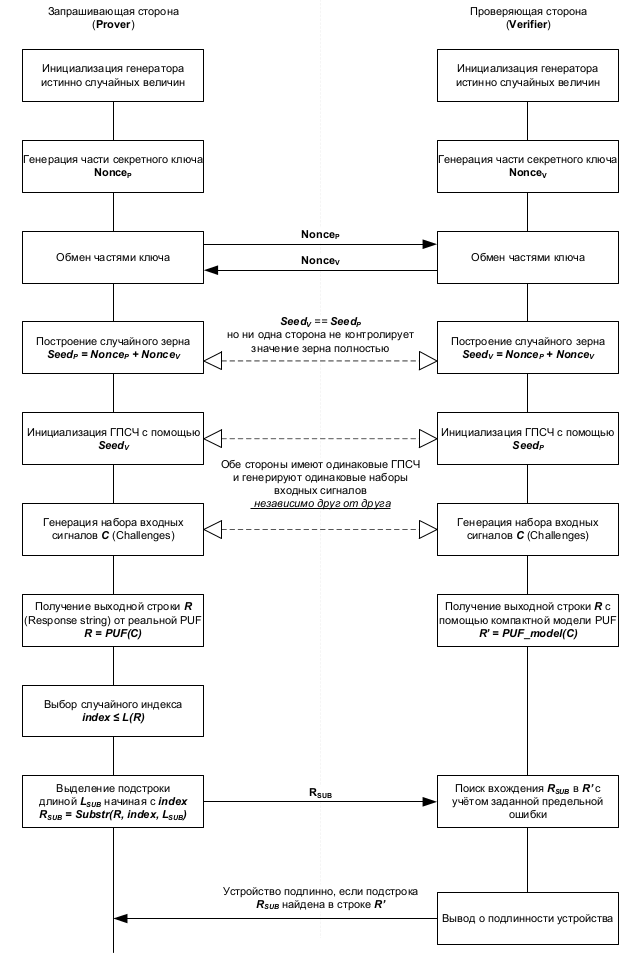
\includegraphics[width=0.93\textwidth]{protocol.png}
    \caption{Схема протокола аутентификации}
    \label{fig:architecture:protocol}
\end{figure}
% }

\clearpage
Набор функций, реализованных в библиотеке, напрямую определяется требованиями протокола. Библиотека предоставляет следующий функционал, используемый как клиентской, так и серверной частью:
\begin{itemize}
  \item Класс-обёртка TRNG для генерации истинно случайных значений с использованием системного генератора случайных чисел. Например в ОС Linux таковым является специальное устройство \emph{/dev/urandom}, предоставляющее интерфейс к пулу случайной информации, сгенерированной драйверами устройств путём сбора метрик шумовых процессов, протекающих при их работе. Применительно к протоколу TRNG используется для получения случайного зерна для PRNG и случайного индекса выходной подпоследовательности в режиме аутентификации и генерации запросов \emph{Challenge} для обучения модели в режиме регистрации.
  \item Класс-обёртка PRNG для генерации псевдослучайных значений. Использует реализацию алгоритма вихря Мерсенна из стандартной библиотеки языка Python. Требует инициализации с помощью зерна. PRNG используется для генерации запросов \emph{Challenge} в режиме аутентификации.
  \item Абстрактный класс Party для обозначения участников взаимодействия по протоколу. Предоставляет реализующим его классам функционал, общий для всех участников: методы идентификации в системе, методы обмена частями случайного зерна, методы генерации псевдослучайных последовательностей входных запросов.
  \item Класс Verifier, реализующий абстрактный класс Party. Представляет сущность сервера проверки подлинности и содержит методы для этапов протокола, специфичных для проверяющей стороны.
  \item Класс Prover, реализующий абстрактный класс Party. Представляет сущность клиентского приложения, представляющего устройство и содержит методы для этапов протокола, специфичных для стороны, запрашивающей проверку.
  \item Класс Configuration, представляющий собой набор конфигурационных параметров протокола и поддерживает инициализацию с помощью файла настроек или системных переменных окружения в дополнение к инициализации с помощью стандартных параметров конструктора.
\end{itemize}

Класс Configuration разобран чуть подробнее, так как от правильного его использования зависит применение параметров работы протокола, влияющих главным образом, на процент ложных срабатываний или наоборот, ложных отказов.
\clearpage
\lstinputlisting[
    style=commonstyle,
    firstline=5,
    caption={Класс Configuration},
    label=lst:architecture:configuration
]{src/configuration.py}

В таблице \ref{table:architecture:cfg_items} приведены краткие описания доступных параметров:

\begin{table}[ht]
  \caption{Параметры протокола аутентификации}
  \label{table:architecture:cfg_items}
  \begin{tabular}{| >{\raggedright}m{0.45\textwidth}
                  | >{\raggedright\arraybackslash}m{0.5\textwidth}|}
   \hline
   Параметр & Описание
   \\ \hline
   \textit{NONCE\_SIZE} & Длина (в битах) половины случайного зерна (результирующее зерно будет иметь длину \textit{2xNONCE\_SIZE}), используемого для инициализации ГПСЧ
   \\ \hline
   \textit{SUBSTR\_LEN} & Длина (в битах) извлекаемой из ответа реального устройства подстроки
   \\ \hline
   \textit{THRESHOLD} & Максимальное значение расстояния Хэмминга между строками, при котором они всё еще считаются схожими
   \\ \hline
   \textit{RSP\_LEN} & Фиксированная длина (в битах) ответа устройства (используется только для тестирования!)
   \\ \hline
  \end{tabular}
\end{table}

В следующих подразделах будут рассмотрены две стороны, взаимодействующие в рамках протокола.

\subsection{Модуль контроля доступа (клиентская часть)}
Так как протокол аутентификации по сути является набором правил, регулирующих обмен информацией нескольких сторон (в данном случае двух), логично описать правила поведения каждой из сторон по отдельности. В реализуемом протоколе участвуют \emph{клиент} -- сторона, имеющая доступ к устройству и <<представляющая его интересы>> в процессе аутентификации и \emph{сервер} -- сторона, обладающая подтверждение подлинности устройства.

В данной упрощённой реализации клиент также контролирует доступ к ресурсу, запрашиваемому устройством. Простейший пример -- электронный ключ в виде устройства с PUF запрашивает доступ к некоторому ресурсу, защищённому электронным замком. Электронный замок ничего не знает о подлинности устройства, в свою очередь устройство не может в одиночку доказать свою подлинность, т.к. по умолчанию не является доверенным. Здесь устройство пользуется <<услугой>> клиента (Prover), который является посредником между устройством, доказывающим свою подлинность, и доверенным сервером, обладающим релевантной информацией насчёт неё. Посредник также контролирует электронный замок, т.е. контролирует, какие устройства могут иметь к секретному ресурсу по результатам процесса аутентификации. Совмещение ролей посредника и барьера, конечно же, не является обязательным и сделано для упрощения архитектуры программного средства и эти роли могут быть без особых проблем разделены для более тонкого контроля над всей инфраструктурой.

По правилам протокола аутентификации клиентский модуль выполняет следующие функции:
\begin{itemize}
  \item генерировать истинно случайные и псевдослучайные данные для использования в алгоритмах протокола;
  \item взаимодействовать с устройством, посылая наборы входных сигналов и считывая результаты на выходе;
  \item создавать компактную модель уPUF на этапе регистрации;
  \item взаимодействовать с сервером, обмениваясь с ним секретной информацией -- с помощью библиотеки requests и грамотного использования защищенных соединений  и клиентских сессий.
\end{itemize}

С добавлением роли барьера примешиваются дополнительно функции надёжного хранения ссылки на секретный ресурс и предоставления устройству ссылки на секретный ресурс  в случае успешной аутентификации.

Как можно увидеть, модуль клиентской стороны использует множество ранее описанных классов и функций, не описывая своих классов или структур данных. Основной задачей клиентского модуля является реализация алгоритма проведения операций регистрации и атуентификации с использованием уже созданных инструментов. В таблице~\ref{table:architecture:client_funcs} описано, как реализованы эти инструменты, на основе которых построен алгоритм, являющийся главной логикой клиентского модуля.

\begin{table}[ht]
  \caption{Функции клиентского модуля и их реализации}
  \label{table:architecture:client_funcs}
  \begin{tabular}{| >{\raggedright}m{0.45\textwidth}
                  | >{\raggedright\arraybackslash}m{0.5\textwidth}|}
   \hline
   Функция & С помощью чего реализована
   \\ \hline
   Генерация истинно случайных чисел & Класс TRNG модуля протокола аутентификации
   \\ \hline
   Генерация псевдослучайных чисел & Класс PRNG модуля протокола аутентификации
   \\ \hline
   Обмен битовыми строками входных и выходных сигналов с утройствами & Класс Device и его производные классы в слое взаимодействия с устройствами
   \\ \hline
   Создание компактной модели PUF & Класс-обёртка над модулем построения модели (для обеспечения интероперабельности языков Python и Haskell)
   \\ \hline
   Контроль доступа у секретным ресурсам & Внутренние функции модуля или опциональный внешний интерфейс.
   \\ \hline
  \end{tabular}
\end{table}

\subsection{Модуль проверки подлинности (серверная часть)}
В описанном выше протоколе \emph{сервер} является сущностью, располагающей информацией о подлинности зарегистрированных устройств. Эта информация представлена в виде компактных моделей PUF, созданных на этапе их регистрации.

Функционал сервера во многом повторяет таковой у клиента, именно поэтому было принято решение вынести общие функции в абстрактный класс Prover. Сервер использует свою реализацию этого класса -- Verifier.

На основании вышесказанного, серверный модуль проверки подлинности выполняет следующие функции:
\begin{itemize}
  \item генерировать истинно случайные и псевдослучайные данные для использования в алгоритмах протокола;
  \item взаимодействовать с моделью устройства, посылая наборы входных сигналов и считывая результаты на выходе;
  \item иметь доступ к хранилищу моделей PUF;
  \item использовать алгоритм нечеткого поиска строки для сравнения данных, полученных от реального устройства с данными, полученными от компактной модели;
  \item работать в режиме сервера, т.е. принимать и обрабатывать входящие запросы, все время находясь в ожидании новых запросов;
\end{itemize}


\lstinputlisting[
    style=commonstyle,
    firstline=18,
    caption={Метод нечеткого поиска подстроки с заданным порогом},
    label=lst:architecture:fuzzysearch
]{src/fulllisting/puf.py}

\begin{table}[ht]
  \caption{Функции серверного модуля и их реализации}
  \label{table:architecture:client_funcs}
  \begin{tabular}{| >{\raggedright}m{0.45\textwidth}
                  | >{\raggedright\arraybackslash}m{0.5\textwidth}|}
   \hline
   Функция & С помощью чего реализована
   \\ \hline
   Работа в качестве HTTP-сервера по защищенному протоколу & Веб-фреймворка Flask и его поддержка безопасных соединений и клиентских сессий.
   \\ \hline
   Генерация истинно случайных чисел & Класс TRNG модуля протокола аутентификации
   \\ \hline
   Генерация псевдослучайных чисел & Класс PRNG модуля протокола аутентификации
   \\ \hline
   Обмен битовыми строками входных и выходных сигналов с моделью PUF & Класс Model
   \\ \hline
   Работа с хранищилем моделей PUF & Класс Database и его реализации для работы с файловой системой, Redis или MongoDB
   \\ \hline
   Нечеткий поиск подстроки & Класс Response модуля PUF и его реализации нечеткого поиска
   \\ \hline
  \end{tabular}
\end{table}


Сервер проверки подлинности должен иметь возможность обмена данными с моделью образом, похожим на способ взаимодействия с устройствами для модуля контроля доступа. Для данной цели создан класс Model, который предоставляет такой же интерфейс к модели PUF, какой предоставляет слой взаимодействия с устройствами для реальных PUF. Метод \emph{f} класса Model принимает масиив битов класса Challenge и возвращает бит ответа -- объект класса Response.

Для взаимодействия с хранилищем моделей модуль проверки подлинности предоставляет простой класс Database, по умолчанию реализующий хранение моделей в виде файлов на файловой системе. В то время как такой подход может быть полезен при тестировании приложения, для реального использования стоит также рассмотреть другие варианты:
\begin{itemize}
  \item NoSQL база данных. Так как модели PUF являются независимыми наборами векторов, использование классической реляционной базы данных в данном случае нерационально, ведь модели не имеют множества атрибутов, как не имеют и связей и отношений с другими сущностями в БД. В рамках этого варианта программное средство поддерживает работу с нереляционной СУБД MongoDB.
  \item Кэш (неперсистентное хранилище). В зависимости от требований информационной системы, в которой планируется использование данного ПС, является вероятным сценарий того, что модели PUF не должны храниться в базе слишком долго, или даже могут являться одноразовыми. В данном случае можно использовать систему хранения временных данных в памяти (memcached, Redis). Более того, так как в системе принято условие <<одно устройство -- одна модель>>, можно обойтись простейшим хранилищем типа <<ключ-значение>>(\emph{key-value store}). Для этого варианта реализован класс для работы с хранилищем Redis.
\end{itemize}
 %

% Глава 4 Тестирование программного средства
\section{Тестирование программного средства}
\label{sec:testing}

Программное средство разрабатывалось в виде набора библиотек. Для использования программной системы необходимо взаимодействие с внешними устройствами, и драйвер, реализуюший этот функционал. Тестирование приложеня предполагает проверку работоспособности самой библиотеки независимо от используемого драйвера. Поэтому перед началом тестирования необходимо произвести следующие подготовительные действия:
\begin{enumerate}
  \item корректно сконфигурировать серверную часть приложения;
  \item на клиентской стороне подключить необходимые библиотеки из состава программной системы;
  \item инициализировать слой взаимодействия с устройствами;
  \item инициировать протокол регистрации или аутентификации устройства в системе.
\end{enumerate}

Тестирование предполагает наличие файлов конфигурации и файла инициализации. В качестве устройства-субъекта аутентификации на этапе тестирования используется программная симуляция ФНФ для обеспечения однозначости и повторяемости результатов тестов.

Для оценки правильности работы программного средства было проведено тестирование. В данном разделе приведены тест-кейсы и их результаты в вид таблиц.

\begin{longtable}[l]{| >{\raggedright}p{0.3\textwidth}
                     | >{\raggedright}p{0.3\textwidth}
                     | >{\raggedright\arraybackslash}p{0.3\textwidth}|}
  \caption{Тестирование доступа к базе моделей устройств}
  \label{table:testing:db}\\
  \endfirsthead
  \caption*{Продолжение таблицы \ref{table:testing:db}}\\
  \endhead

  \hline
       Название тест-кейса и его описание & Ожидаемый результат & Фактический результат \\
   \hline
   Получение модели PUF по id устройства \\
   1) Инициализировать объект класса Database; \\
   2) вызвать функцию Database.get с id зарегистрированного устройства в качестве параметра.
   &
   1) Объект класса Database сигнализирует об успешной инициализации; \\
   2) результатом функции является объект класса Model с параметром id, использованным в запросе.
   &
   Тест пройден \\ \hline

\end{longtable}

\begin{longtable}[l]{| >{\raggedright}p{0.3\textwidth}
                     | >{\raggedright}p{0.3\textwidth}
                     | >{\raggedright\arraybackslash}p{0.3\textwidth}|}
  \caption{Тестирование программы построения компактной модели PUF}
  \label{table:testing:bayes}\\
  \endfirsthead
  \caption*{Продолжение таблицы \ref{table:testing:bayes}}\\
  \endhead

  \hline
       Название тест-кейса и его описание & Ожидаемый результат & Фактический результат \\
   \hline
   Запуск обучения модели из файла \\
   1) В интерфейсе коммандной строки набрать путь исполняемого файла и путём к файлу данных; \\
   2) нажать клавишу ввода и ожидать завершения программы.
   &
   1) Имя исполняемого модуля и путь к файлу отображаются в консоли; \\
   2) отображается результат обучения модели в виде вектора апостериорных вероятностей.
   &
   Тест пройден \\ \hline

   Запуск обучения модели из файла с заданным количеством попыток \\
   1) В интерфейсе коммандной строки набрать путь исполняемого файла модуля с путём к файлу векторов данных и числом попыток обучения модели в качестве аргументов; \\
   2) нажать клавишу ввода и ожидать завершения программы.
   &
   1) Имя исполняемого модуля, путь к файлу и число попыток обучения отображаются в консоли; \\
   2) отображаются обученные модели в количестве, равном числу попыток, и отмечается модель с наименьшим процентом ошибок.
   &
   Тест пройден \\

   \hline
\end{longtable}

Далее тестируется запуск сервера с заданной конфигурацией? котороя может быть представлена в виде ini-файла или с описана с помощью перемеженных окружения.
\clearpage

\begin{longtable}[l]{| >{\raggedright}p{0.3\textwidth}
                     | >{\raggedright}p{0.3\textwidth}
                     | >{\raggedright\arraybackslash}p{0.3\textwidth}|}
  \caption{Тестирование программы построения компактной модели PUF}
  \label{table:testing:servercfg}\\
  \endfirsthead
  \caption*{Продолжение таблицы \ref{table:testing:servercfg}}\\

  \hline
       Название тест-кейса и его описание & Ожидаемый результат & Фактический результат \\
  \endhead
   \hline
   Запуск сервера с настройками по умолчанию \\
   1) В коммандной строки набрать команду запуска сервера; \\
   2) нажать клавишу ввода.
   &
   1) Имя скрипта запуска сервера отображаются в консоли; \\
   2) отображается диагностическая информация о запуске сервера и предустановленных параметра функционирования.
   &
   Тест пройден \\ \hline

   Запуск сервера с настройками из ini-файла \\
   1) В коммандной строки набрать команду запуска сервера и путь к ini-файлу в качестве аргумента; \\
   2) нажать клавишу ввода.
   &
   1) Имя скрипта запуска сервера отображаются в консоли; \\
   2) отображается диагностическая информация о запуске сервера и параметра функционирования, взятых из преоставленного ini-файла.
   &
   Тест пройден \\ \hline
\end{longtable}

\clearpage
\begin{longtable}[l]{| >{\raggedright}p{0.3\textwidth}
                     | >{\raggedright}p{0.3\textwidth}
                     | >{\raggedright\arraybackslash}p{0.3\textwidth}|}
  \caption{Тестирование взаимодействия с уcтройством}
  \label{table:testing:pufbit}\\
  \endfirsthead
  \caption*{Продолжение таблицы \ref{table:testing:pufbit}}\\
  \endhead

  \hline
       Название тест-кейса и его описание & Ожидаемый результат & Фактический результат \\
   \hline
   Использование функции PUF для получения выходного бита \\
   1) Инициировать экземпляр класса Prover c объектом Device в качестве аргумента; \\
   2) сгенерировать случайный объект Challenge с помощью объекта Prover; \\
   3) запустить функцию Device.f с аргументом Challenge.
   &
   1) Объект класса Prover возвращает статус успешной инициализации; \\
   2) объект Challenge является битовой строкой из случайных нулей и единиц; \\
   3) значением функции является случайный бит 0 или 1.
   &
   Тест пройден \\ \hline

   Использование модели функции PUF для получения выходного бита \\
   1) Инициировать экземпляр класса Verifier c объектом Device в качестве аргумента; \\
   2) сгенерировать случайный объект Challenge с помощью объекта Verifier; \\
   3) запустить функцию Model.f с аргументом Challenge.
   &
   1) Объект класса Verifier возвращае статус успешной инициализации; \\
   2) объект Challenge является битовой строкой из случайных нулей и единиц; \\
   3) значением функции является случайный бит 0 или 1.
   &
   Тест пройден \\ \hline

   \hline
\end{longtable}

\clearpage

В следующих таблицах(\ref{table:testing:proto} и \ref{table:testing:regpuf}) тестируются два основных режима: режим регистрации и режим аутенификации, при тестировании которого проверятся также случай, когда злоумышленником прелпринимается попытка аутентификации с помощью поддельного PUF. Даже случае подмены идентификатора устройства решение о предоставлении доступа будет принято на основе соответствия поведения устройства поведению зарегистрированной модели.


\begin{longtable}[l]{| >{\raggedright}p{0.3\textwidth}
                     | >{\raggedright}p{0.3\textwidth}
                     | >{\raggedright\arraybackslash}p{0.3\textwidth}|}
  \caption{Тестирование протокола аутентификации}
  \label{table:testing:proto}\\
    \hline
       Название тест-кейса и его описание & Ожидаемый результат & Фактический результат \\
    \hline
  \endfirsthead
  \caption*{Продолжение таблицы \ref{table:testing:proto}}\\

  \hline
       Название тест-кейса и его описание & Ожидаемый результат & Фактический результат \\
   \hline
  \endhead
  \endlastfoot
   Аутентификация незарегистрированного устройства \\
   1) Инициировать объект класса Device, связанного с незарегистрированным устройством; \\
   2) подменить поле id объекта Device, на id, связанный с зарегистрированным устройством; \\
   3) инициировать экземпляр класса Prover c объектом Device и адресом сервера аутентификации в качестве аргументов; \\
   4) вызвать функцию Prover.authenticate.
   &
   1) Объект класса Device имеет id незарегистрированного устройства; \\
   2) объект класса Device имеет id зарегистрированного устройства; \\
   3) объект класса Prover возвращает статус успешной инициализации; \\
   4) сервер возвращает сообщение об отклонение запроса и предупреждение о поддельном устройстве.
   &
   Тест пройден \\

   Аутентификация подлинного устройства \\
   1) Инициировать объект класса Device, связанного с зарегистрированным устройством; \\
   2) инициировать экземпляр класса Prover c объектом Device и адресом сервера аутентификации в качестве аргументов; \\
   3) вызвать функцию Prover.authenticate.
   &
   1) Объект класса Device имеет id зарегистрированного устройства; \\
   2) объект класса Prover возвращает статус успешной инициализации; \\
   3) сервер возвращает сообщение об успешной аутентификации.
   &
   Тест пройден \\
   \hline


\end{longtable}


\begin{longtable}[l]{| >{\raggedright}p{0.3\textwidth}
                     | >{\raggedright}p{0.3\textwidth}
                     | >{\raggedright\arraybackslash}p{0.3\textwidth}|}
  \caption{Тестирование регистрации устройства}
  \label{table:testing:regpuf}\\
  \endfirsthead
  \caption*{Продолжение таблицы \ref{table:testing:regpuf}}\\
  \endhead

  \hline
       Название тест-кейса и его описание & Ожидаемый результат & Фактический результат \\
   \hline
   Регистрация устройства в базе данных \\
   1) Инициировать экземпляр класса Prover c объектом Device в качестве аргумента; \\
   2) вызвать функцию Prover.register. \\
   &
   1) Объект класса Prover возвращает статус успешной инициализации; \\
   2) сервер возвращает сообщение об успешной регистрации.
   &
   Тест пройден \\ \hline
\end{longtable}
 %

% Глава 5 Использование разработанного программного средства
\section{Методика использования программной системы}
\label{sec:manpage}

Программное средство распознавания уникальных неклонируемых идентификаторов цифровых устройств является комплексным продуктом и рассчитано на работу по схеме клиент-сервер. Ниже приведен возможный вариант развертывания и конфигурации программной системы.

\subsection{Настройка сервера}
\label{sec:manpage:server_setup}
Модуль проверки подлинности (сервер) может запускаться в одиночном режиме как обычное Python-приложение. Однако, такой подход не является рекомендованным и не обеспечивает достаточную секретность информации и стабильность системы. Сервер аутентификации рассчитан на работу в связке с WSGI-сервером и веб-сервером. Возможная схема их подключения показана на рисунке \ref{fig:manpage:nginx_proxy}.

\begin{figure}[!h]
    \centering
    \includegraphics[width=0.65\textwidth]{nginx_proxy.png}
    \caption{Схема возможного развертывания приложения в связке с WSGI-сервером и HTTP-сервером}
    \label{fig:manpage:nginx_proxy}
\end{figure}


Для обеспечения лучшей совместимости программных компонентов рекомендуется развертывание на устройствах под управением операционной системы семейства Linux. В листингах \ref{lst:manpage:gunicorncfg} и \ref{lst:manpage:nginxcfg} приведен пример рекомендуемой конфигурации менеджера процессов \emph{systemd} для запуска WSGI-сервера \emph{gunicorn} и настроек HTTP-сервера \emph{nginx} соответственно.


Программное средство рассчитано на работу по протоколу HTTPS в целях обеспечения секретности передаваемой информации. Для развертывания внутри закрытой сети достаточно использования самоподписанного (\emph{self-signed}) SSL/TLS"=сертификата, однако, если сценарий использования предполагает прохождение информационных потоков через публичные сети, например, Интернет, крайне рекомендуется использование валидного сертификата, подписанного доверенным центром сертификации. В обоих случаях необходимо правильная настройка сетевого экрана, для исключения перехвата данных или осуществления атаки отказа в обслуживании (DDoS) злоумышленником. При использовании вышеописанного сценария развертывания, достаточно разрешения входящего и исходящего трафика по стандартному HTTPS-порту 443.


\lstinputlisting[
    style=commonstyle,
    caption=Пример конфигурации systemd для запуска приложения в связке с WSGI-сервером gunicorn,
    label=lst:manpage:gunicorncfg
]{src/systemdgunicorn.conf}

\lstinputlisting[
    style=commonstyle,
    caption=Пример конфигурации nginx в качестве прокси-сервера,
    label=lst:manpage:nginxcfg
]{src/nginx.conf}

В целом, настройка и развертывание серверной части ничем не отличается от развертывания любого другого Python/WSGI-приложения, поэтому связанные с ними нюансы не являются частью данного руководства.

\subsection{Настройка модуля контроля доступа}
\label{sec:manpage:client_setup}
Модуль контроля доступа (Prover) является посредником между устройством и сервером аутентификации. Он не хранит секретных данных, однако может взаимодействать с реальными устройствами, поэтому он также должен быть развернут в безопасном окружении. Модуль контроля доступа сообщается с модулем проверки подлинности по протоколу HTTPS, как показано на рисунке \ref{fig:manpage:nginx_proxy}.


\subsection{Пример использования}
Программное средство поддерживает два этапа взаимодействия устройства с информационной системой -- регистрацию и аутентификацию. Для обеих целей в состав ПС входят утилиты \emph{register\_device.py} и \emph{authenticate\_device.py}. Они предоставляют базовый функционал и носят скорее демонстрационный характер, так как ПС рассчитана на интеграцию с существующей системой безопасности и предоставляет API для реализации нужд этой системы. Исходный код утилит представлен в листингах \ref{lst:manpage:authdev} и \ref{lst:manpage:regdev}.

\lstinputlisting[
    style=commonstyle,
    caption=Вспомогательный скрипт аутентификации утсройства,
    label=lst:manpage:authdev
]{src/authenticate_device.py}

\lstinputlisting[
    style=commonstyle,
    caption=Вспомогательный скрипт регистрации утсройства,
    label=lst:manpage:regdev
]{src/register_device.py}

\subsection{Расширение функциональности программного средства}
Программное средство может быть расширено для обеспечения поддержки различных типов устройств и подключений. Базовая поставка программной системы включает программную симуляцию PUF-устройства типа арбитр и класс (драйвер) для работы с ним. Добавление новых драйверов происходит путем переопределения базового класса devices.Device и реализации метода создания виртуального объекта устройства и собственного метода функции PUF, предназначенного для передачи входного сигнала устройству и получения выходного.

\lstinputlisting[
    style=commonstyle,
    caption={Пример переопределения класса Device для работы с программной реализацией PUF-арбитра},
    label=lst:architecture:software_arbiter
]{src/fulllisting/software_arbiter.py}
 %

% Глава 6 Технико-экономическое обоснование разработки ПС
\def \byr{Br}

\section{Технико-экономическое обоснование разработки ПС}

% Категория сложности
\def \complexityGroup{3}

% Категория новизны
\def \noveltyGroup{Б}

% ---

Целью дипломного проектирования является создание программного средства для распознавания уникальных идентификаторов цифровых устройств с целью их аутентификации. Данное ПС реализует протокол аутентификации на основе использования и анализа информации, полученной от специального компонента цифрового устройства, выполненного в виде физически неклонируемой функции (ФНФ). Использование ФНФ позволяет добиться целостности и неклонируемости идентификатора устройства и однозначности при проверке подлинности устройства. Основными достоинствами программного средства являются: высокая производительность при низких системных требованиях; модульная архитектура, разделяющая взаимодействие с устройством и собственно обработку идентификационных данных и аутентификацию.

В данном разделе рассмотрим экономическую эффективность программного средства.  Программный комплекс относится к \complexityGroup-й группе сложности. Категория новизны продукта – <<\noveltyGroup>>. Для оценки экономической эффективности разработанного программного средства необходимо рассчитать смету затрат на разработку, цену и прибыль продажи одной программной системы.

Расчеты выполнены на основе методического пособия ~\cite{palicyn_2006}.



\subsection{Расчёт сметы затрат и цены программного продукта}

% Коэффициент сложности, ед.
\def \additionalComplexityFactor{0.12}
\FPeval{complexityFactor}{clip(1 + \additionalComplexityFactor)}

% Степень использования при разработке стандартных модулей, ед.
\def \stdModuleUsageFactor{0.6}

% Коэффициент новизны, Кн
\def \noveltyFactor{0.9}

% Годовой эффективный фонд времени, дн.
\def \daysInYear{366}
\def \holidaysInYear{6}
\def \weekendDaysInYear{105}
\def \vacationDaysInYear{24}
\FPeval{workingDaysInYear}{
    clip(\daysInYear -
         \holidaysInYear -
         \weekendDaysInYear -
         \vacationDaysInYear)
}

% Среднемесячная норма рабочего времени, Фр
\def \workingHoursInMonth{160}

% Продолжительность рабочего дня, ч.
\def \workingHoursInDay{8}

% Месячная тарифная ставка первого разряда, Br
% \def \tariffRate{298000} % Гос. предприятия
\def \tariffRate{1150000}

% Коэффициент премирования, ед
\def \bonusRate{1.5}

% Норматив дополнительной заработной платы, Br
\def \additionalSalaryRate{20}

% Норматив отчислений в ФСЗН и обязательное страхование, %
\def \socialProtectionRate{34}

% Норматив отчислений в Белгосстрах
\def \bgsRate{0.7}

% Норматив командировочных расходов, %
\def \businessTripRate{15}

% Норматив прочих затрат, %
\def \otherExpenseRate{20}

% Норматив накладных расходов, %
\def \overheadExpenseRate{100}

% Прогнозируемый уровень рентабельности, %
\def \profitability{35}

% Норматив отчислений в местный и республиканский ю.джет
\def \localRepubTaxRate{3.9}

% Норматив НДС, %
\def \vatRate{20}

% Норматив налога на прибыль, %
\def \profitTaxRate{18}

% Норматив расхода материалов, %
\def \materialsRate{3}

% Норматив расхода машинного времени, ч.
\def \debugRate{15} % часов / 100 строк кода

% Цена одного часа машинного времени, Br
\def \machineHourCost{25000}

% Норматив расходов на сопровождение и адаптацию ПО, %
\def \supportAndAdaptationRate{30}

% ---

Исходные данные для разрабатываемого проекта указаны в таблице~\ref{table:economics:initial_data}.

\begin{longtable}{| >{\raggedright}m{0.62\textwidth}
                  | >{\centering}m{0.17\textwidth}
                  | >{\centering\arraybackslash}m{0.13\textwidth}|}
    \caption{Исходные данные}
    \label{table:economics:initial_data}
    \\

    \hline
    {\begin{center} Наименование \end{center} } & Условное обозначение & Значение
    \\ \hline

    Категория сложности
    & & \complexityGroup
    \\ \hline

    Коэффициент сложности, ед.
    & $ \text{К}_\text{с} $ & \num{\complexityFactor}
    \\ \hline

    Степень использования при разработке стандартных модулей, ед.
    & $ \text{К}_\text{т} $ & \num{\stdModuleUsageFactor}
    \\ \hline

    Коэффициент новизны, ед.
    & $ \text{К}_\text{н} $ & \num{\noveltyFactor}
    \\ \hline

    Годовой эффективный фонд времени, дн.
    & $ \text{Ф}_\text{эф} $ & \num{\workingDaysInYear}
    \\ \hline

    Продолжительность рабочего дня, ч.
    & $ \text{Т}_\text{ч} $ & \num{\workingHoursInDay}
    \\ \hline

    Месячная тарифная ставка первого разряда, \byr{}
    & $ \text{Т}_{\text{м}_{1}}$ & \num{\tariffRate}
    \\ \hline

    Коэффициент премирования, ед.
    & $ \text{К} $ & \num{\bonusRate}
    \\ \hline

    Норматив дополнительной заработной платы, ед.
    & $ \text{Н}_\text{д} $ & \num{\additionalSalaryRate}
    \\ \hline

    Норматив отчислений в ФСЗН, $\%$
    & $ \text{Н}_\text{сз} $ & \num{\socialProtectionRate}
    \\ \hline

    Норматив отчислений в Белгосстрах, $\%$
    & $ \text{Н}_\text{с} $ & \num{\socialProtectionRate}
    \\ \hline

    Норматив командировочных расходов, $\%$
    & $ \text{Н}_\text{к} $ & \num{\businessTripRate}
    \\ \hline

    Норматив прочих затрат, $\%$
    & $ \text{Н}_\text{пз} $ & \num{\otherExpenseRate}
    \\ \hline

    Норматив накладных расходов, $\%$
    & $ \text{Н}_\text{рн} $ & \num{\overheadExpenseRate}
    \\ \hline

    Прогнозируемый уровень рентабельности,
    $\%$ & $ \text{У}_\text{рп} $ & \num{\profitability}
    \\ \hline

    Норматив НДС, $\%$
    & $ \text{Н}_\text{дс} $ & \num{\vatRate}
    \\ \hline

    Норматив налога на прибыль, $\%$
    & $ \text{Н}_\text{п} $ & \num{\profitTaxRate}
    \\ \hline

    Норматив расхода материалов, $\%$
    & $ \text{Н}_\text{мз} $ & \num{\materialsRate}
    \\ \hline

    Норматив расхода машинного времени, ч.
    & $ \text{Н}_\text{мв} $ & \num{\debugRate}
    \\ \hline

    Цена одного часа машинного времени, \byr{}
    & $ \text{Н}_\text{мв} $ & \num{\machineHourCost}
    \\ \hline

    Норматив расходов на сопровождение и адаптацию ПО, $\%$
    & $ \text{Н}_\text{рса} $ & \num{\supportAndAdaptationRate}
    \\ \hline
\end{longtable}

На основании сметы затрат и анализа рынка ПО определяется плановая отпускаемая цена.
Для составления сметы затрат на создание ПО необходима предварительная оценка трудоемкости ПО и его объёма.
Расчет объёма программного продукта (количества строк исходного кода) предполагает определение типа программного обеспечения, всестороннее техническое обоснование функций ПО и определение объёма каждой функций.
Согласно классификации типов программного обеспечения~\cite[с.~59,~приложение 1]{palicyn_2006}, разрабатываемое ПО с наименьшей ошибкой можно классифицировать как ПО методo"=ориентированных расчетов.

Общий объём программного продукта определяется исходя из количества и объёма функций, реализованных в программе:
\begin{equation}
  \label{eq:economics:total_loc}
  V_{o} = \sum_{i = 1}^{n} V_{i} \text{\,,}
\end{equation}
\begin{explanation}
где & $ V_{i} $ & объём отдельной функции ПО, LoC; \\
    & $ n $ & общее число функций.
\end{explanation}

На стадии технико-экономического обоснования проекта рассчитать точный объём функций невозможно.
Вместо вычисления точного объёма функций применяются приблизительные оценки на основе данных по аналогичным проектам или по нормативам~\cite[с.~61,~приложение 2]{palicyn_2006}, которые приняты в организации.

\def \totalLOC{9710} % TODO
\def \totalLOCCorrected{6390} % TODO

\begin{longtable}{| >{\centering}m{0.12\textwidth}
                  | >{\raggedright}m{0.40\textwidth}
                  | >{\centering}m{0.18\textwidth}
                  | >{\centering\arraybackslash}m{0.18\textwidth}|}
  \caption{Перечень и объём функций программного модуля}
  \label{table:econ:function_sizes}
  \\

  \hline
    \multirow{2}{0.12\textwidth}[-0.5em]{\centering \No{} функции}
    & \multirow{2}{0.40\textwidth}[-0.55em]{\centering Наименование (содержание)}
    & \multicolumn{2}{c|}{\centering Объём функции, LoC} \tabularnewline

  \cline{3-4} &
       & { по каталогу ($ V_{i} $) }
       & { уточненный ($ V_{i}^{\text{у}} $) } \tabularnewline
  \hline

  101 & Организация системы подключаемых модулей
  & \num{620} & \num{450}
  \\ \hline

  102 & Контроль, предварительная обработка и ввод информации
  & \num{450} & \num{300}
  \\ \hline

  111 & Обработка исходных данных и тренировка математической модели
  & \num{3100} & \num{1900}
  \\ \hline

  301 & Интерфейс к базе данных моделей и данных аутентификации
  & \num{790} & \num{650}
  \\ \hline

  305 & Защита от несанкционированного доступа к базе
  & \num{820} & \num{400}
  \\ \hline

  501 & Монитор ПО (управление работой компонентов)
  & \num{1240} & \num{910}
  \\ \hline

  506 & Обработка исключительных ситуаций
  & \num{620} & \num{400}
  \\ \hline

  507 & Обеспечение интерфейса между компонентами
  & \num{970} & \num{680}
  \\ \hline

  612 & Аутентификация на основе сравнения реальных данных и математической модели
  & \num{1100} & \num{700}
  \\ \hline

  Итог & &
  {\num{\totalLOC}} & {\num{\totalLOCCorrected}}
  \\ \hline

\end{longtable}

Перечень и объём функций программного модуля перечислен в таблице~\ref{table:econ:function_sizes}.
По приведенным данным уточненный объём некоторых функций изменился, и общий уточненный объём ПО
$ V_{\text{у}} = \SI{\totalLOCCorrected}{\text{LoC}} $
.



\subsection{Расчёт трудоемкости}

% Нормативная трудоёмкость, Тн
\def \normativeWorkload{144}

% Общая трудоёмкость, То
\FPeval{totalWorkload}{
    trunc(\normativeWorkload *
          \complexityFactor *
          \stdModuleUsageFactor *
          \noveltyFactor + 0.5, 0)
}

% Срок разработки проекта, Тр
\def \developmentMonths{3}
\FPeval{developmentYears}{round(\developmentMonths / 12, 2)}

% Численность исполнителей, Чр
\FPeval{requiredProgrammers}{trunc(\totalWorkload / (\developmentYears * \workingDaysInYear) + 0.5, 0) }

% Считаем, что работы каждому достаётся поровну.
\FPeval{workloadSenior}{trunc( \totalWorkload / \requiredProgrammers, 0 )}
\FPeval{workloadLead}{clip(\totalWorkload - \workloadSenior)}

% ---

На основании общего объема ПО определяется нормативная трудоемкость (
$ \text{Т}_\text{н}$
) с учетом сложности ПО. Для ПО \complexityGroup-ой группы сложности, к которой относится разрабатываемый программный продукт, нормативная трудоемкость составит~
$ \text{Т}_\text{н} = \SI{\normativeWorkload}{\text{чел.} / \text{дн.}} $

Нормативная трудоемкость служит основой для оценки общей трудоемкости~
$ \text{Т}_\text{о} $
.
Используем формулу (\ref{eq:economics:total_workload}) для оценки общей трудоемкости для небольших проектов:
\begin{equation}
  \label{eq:economics:total_workload}
  \text{Т}_\text{о} = \text{Т}_\text{н} \cdot
                      \text{К}_\text{с} \cdot
                      \text{К}_\text{т} \cdot
                      \text{К}_\text{н} \text{\,,}
\end{equation}
\begin{explanation}
где & $ \text{К}_\text{с} $ & коэффициент, учитывающий сложность ПО; \\
    & $ \text{К}_\text{т} $ & поправочный коэффициент, учитывающий степень использования при разработке стандартных модулей; \\
    & $ \text{К}_\text{н} $ & коэффициент, учитывающий степень новизны ПО.
\end{explanation}

Дополнительные затраты труда на разработку ПО учитываются через коэффициент сложности, который вычисляется по формуле
\begin{equation}
\label{eq:economics:additional_complexity_factor}
  \text{К}_{\text{с}} = 1 + \sum_{i = 1}^n \text{К}_{i} \text{\,,}
\end{equation}
\begin{explanation}
где & $ \text{К}_{i} $ & коэффициент, соответствующий степени повышения сложности ПО за счет конкретной характеристики; \\
    & $ n $ & количество учитываемых характеристик.
\end{explanation}

Наличие двух характеристик сложности позволяет~\cite[c.~66, приложение~4, таблица~П.4.2]{palicyn_2006} вычислить коэффициент сложности
\begin{equation}
\label{eq:economics:complexity_factor}
  \text{К}_{\text{с}} = \num{1} + \num{\additionalComplexityFactor} = \num{\complexityFactor} \text{\,.}
\end{equation}

Разрабатываемое ПО использует стандартные компоненты. Согласно справочным данным~\cite[c.~68,~приложение~4, таблица~П.4.5]{palicyn_2006} коэффициент использования стандартных модулей для разрабатываемого приложения
$ \text{К}_\text{т} = \num{\stdModuleUsageFactor} $
.

Согласно справочным данным~\cite[c.~67, приложение~4, таблица~П.4.4]{palicyn_2006}, коэффициент новизны для разрабатываемого ПО
$ \text{К}_\text{н} = \num{\noveltyFactor} $
.

Подставив приведенные выше коэффициенты для разрабатываемого ПО в формулу~(\ref{eq:economics:total_workload}) получим общую трудоемкость разработки
\begin{equation}
  \label{eq:economics:total_workload_calc}
  \text{Т}_\text{о} = \num{\normativeWorkload}
                      \times \num{\complexityFactor}
                      \times \num{\stdModuleUsageFactor}
                      \times \num{\noveltyFactor}
                    \approx \SI{\totalWorkload}{\text{чел.}/\text{дн.}}
\end{equation}

На основе общей трудоемкости и требуемых сроков реализации проекта вычисляется плановое количество исполнителей.
Численность исполнителей проекта рассчитывается по формуле:
\begin{equation}
  \label{eq:economics:num_of_programmers}
  \text{Ч}_\text{р} = \frac{\text{Т}_\text{о}}
                           {\text{Т}_\text{р}
                      \cdot \text{Ф}_\text{эф}} \text{\,,}
\end{equation}
\begin{explanation}
где & $ \text{Т}_\text{о} $ & общая трудоемкость разработки проекта, $ \text{чел.}/\text{дн.} $; \\
    & $ \text{Ф}_\text{эф} $ & эффективный фонд времени работы одного работника в течение года, дн.; \\
    & $ \text{Т}_\text{р} $ & срок разработки проекта, лет.
\end{explanation}

Эффективный фонд времени работы одного разработчика вычисляется по формуле
\begin{equation}
  \label{eq:economics:workload_per_programmer}
  \text{Ф}_\text{эф} = \text{Д}_\text{г} -
                       \text{Д}_\text{п} -
                       \text{Д}_\text{в} -
                       \text{Д}_\text{о} \text{\,,}
\end{equation}
\begin{explanation}
где & $ \text{Д}_\text{г} $ & количество дней в году, дн.; \\
    & $ \text{Д}_\text{п} $ & количество праздничных дней в году, не совпадающих с выходными днями, дн.; \\
    & $ \text{Д}_\text{в} $ & количество выходных дней в году, дн.; \\
    & $ \text{Д}_\text{п} $ & количество дней отпуска, дн.
\end{explanation}

Согласно данным, приведенным в производственном календаре для пятидневной рабочей недели в 2016 году для Беларуси~\cite{belcalendar_2016}, фонд рабочего времени составит
\begin{equation}
  \text{Ф}_\text{эф} = \num{\daysInYear} -
                       \num{\holidaysInYear} -
                       \num{\weekendDaysInYear} -
                       \num{\vacationDaysInYear}
                     = \SI{\workingDaysInYear}{\text{дн.}}
\end{equation}

Учитывая срок разработки проекта
$ \text{Т}_\text{р} = \SI{\developmentMonths}{\text{мес.}} = \SI{\developmentYears}{\text{года}} $
, общую трудоемкость и фонд эффективного времени одного работника, вычисленные ранее, можем рассчитать численность исполнителей проекта
\begin{equation}
  \label{eq:econ:num_of_programmers_calc}
  \text{Ч}_\text{р} = \frac{\num{\totalWorkload}}
                           {\num{\developmentYears}
                      \times \num{\workingDaysInYear}}
                    \approx \SI{\requiredProgrammers}{\text{рабочих}}.
\end{equation}

Вычисленные оценки показывают, что для выполнения запланированного проекта в указанные сроки необходимо \requiredProgrammers ~рабочих.



\subsection{Расчёт заработной платы исполнителей}

% Тариффные коэффициенты, Тк
\def \tariffFactorSenior{3.25} % == 14 разряд
\def \tariffFactorLead{3.48}   % == 15 разряд

% Часовая тарифная ставка исполнителей, Тч
\FPeval{hourlySalarySenior}{round( \tariffRate * \tariffFactorSenior / \workingHoursInMonth, 0 )}
\FPeval{hourlySalaryLead}{round( \tariffRate * \tariffFactorLead / \workingHoursInMonth, 0 )}

% Основная арплата, Зо
\FPeval{baseSalary}{
     round(\workingHoursInDay *
           \bonusRate *
           (\hourlySalarySenior * \workloadSenior +
            \hourlySalaryLead * \workloadLead), 0)
}

% Дополнительная зарплата, Зд
\FPeval{additionalSalary}{ round( \baseSalary * \additionalSalaryRate / 100, 0 ) }


% ---

Информация о работниках перечислена в таблице~\ref{table:economics:programmers}.
\begin{table}[ht]
  \caption{Работники, занятые в проекте}
  \label{table:economics:programmers}
  \begin{tabular}{| >{\centering}m{0.4\textwidth}
                  | >{\centering}m{0.15\textwidth}
                  | >{\centering}m{0.18\textwidth}
                  | >{\centering\arraybackslash}m{0.15\textwidth}|}
   \hline
   Исполнители & Разряд & Тарифный коэффициент & \mbox{Чел./дн.} занятости
   \\ \hline

   Программист \Rmnum{1}-категории & $ \num{14} $ & $ \num{\tariffFactorSenior} $ & $ \num{\workloadSenior} $
   \\ \hline
   Ведущий программист & $ \num{15} $ & $ \num{\tariffFactorLead} $ & $ \num{\workloadLead} $
   \\ \hline
  \end{tabular}
\end{table}

Месячная тарифная ставка одного работника вычисляется по формуле
\begin{equation}
  \label{eq:economics:monthly_salary}
  \text{Т}_\text{ч} =
    \frac {\text{Т}_{\text{м}_{1}} \cdot \text{Т}_{\text{к}} }
          {\text{Ф}_{\text{р}} }  \text{\,,}
\end{equation}
\begin{explanation}
где & $ \text{Т}_{\text{м}_{1}} $ & месячная тарифная ставка 1-го разряда, \byr; \\
    & $ \text{Т}_{\text{к}} $ & тарифный коэффициент, соответствующий установленному тарифному разряду; \\
    & $ \text{Ф}_{\text{р}} $ & среднемесячная норма рабочего времени, час.
\end{explanation}


Подставив данные из таблицы~\ref{table:economics:programmers} в формулу~(\ref{eq:economics:monthly_salary}), приняв значение тарифной ставки 1-го разряда
$ \text{Т}_{\text{м}_{1}} = \SI{\tariffRate}{\text{\byr}} $
и среднемесячную норму рабочего времени
$ \text{Ф}_{\text{р}} = \SI{\workingHoursInMonth}{\text{часов}} $
получаем
\begin{equation}
  \label{eq:economics:monthly_salary_senior}
  \text{Т}_{\text{ч}}^{\text{прогр. \Rmnum{1}-разр.}} =
      \frac{ \num{\tariffRate} \times \num{\tariffFactorSenior} }
           { \num{\workingHoursInMonth} }
    = \SI{\hourlySalarySenior}{\text{\byr}/\text{час;}}
\end{equation}
\begin{equation}
  \label{eq:economics:monthly_salary_lead}
  \text{Т}_{\text{ч}}^{\text{вед. прогр.}} =
      \frac{ \num{\tariffRate} \times \num{\tariffFactorLead} }
           { \num{\workingHoursInMonth} }
    = \SI{\hourlySalaryLead}{\text{\byr}/\text{час.}}
\end{equation}

Основная заработная плата исполнителей на конкретное ПО рассчитывается по формуле
\begin{equation}
  \label{eq:economics:base_salary}
  \text{З}_{\text{о}} = \sum^{n}_{i = 1}
                        \text{Т}_{\text{ч}}^{i} \cdot
                        \text{Т}_{\text{ч}} \cdot
                        \text{Ф}_{\text{п}} \cdot
                        \text{К}
                        \text{\,,}
\end{equation}
\begin{explanation}
где & $ \text{Т}_{\text{ч}}^{i} $ & часовая тарифная ставка \mbox{$ i $-го} исполнителя, \byr$/$час; \\
    & $ \text{Т}_{\text{ч}} $ & количество часов работы в день, час; \\
    & $ \text{Ф}_{\text{п}} $ & плановый фонд рабочего времени \mbox{$ i $-го} исполнителя, дн.; \\
    & $ \text{К} $ & коэффициент премирования.
\end{explanation}

Подставив ранее вычисленные значения и данные из таблицы~\ref{table:economics:programmers} в формулу~(\ref{eq:economics:base_salary}) и приняв коэффициент премирования
$ \text{К} = \num{\bonusRate} $
получим
\begin{equation}
  \label{eq:economics:base_salary_calc}
  \text{З}_{\text{о}} = (\hourlySalarySenior \times \num{\workloadSenior} +
                         \hourlySalaryLead \times \num{\workloadLead})
                        \times \num{\workingHoursInDay}
                        \times \num{\bonusRate}
                      = \SI{\baseSalary}{\text{\byr}} \text{\,.}
\end{equation}

Дополнительная заработная плата включает выплаты предусмотренные законодательством от труде и определяется по нормативу в процентах от основной заработной платы
\begin{equation}
  \label{eq:economics:additional_salary}
  \text{З}_{\text{д}} =
    \frac {\text{З}_{\text{о}} \cdot \text{Н}_{\text{д}}}
          {100\%} \text{\,,}
\end{equation}
\begin{explanation}
  где & $ \text{Н}_{\text{д}} $ & норматив дополнительной заработной платы, $ \% $.
\end{explanation}

Приняв норматив дополнительной заработной платы
$ \text{Н}_{\text{д}} = \num{\additionalSalaryRate\%} $
и подставив известные данные в формулу~(\ref{eq:economics:additional_salary}) получим
\begin{equation}
  \label{eq:econ:additional_salary_calc}
  \text{З}_{\text{д}} =
    \frac{\num{\baseSalary} \times 20\%}
         {100\%} \approx \SI{\additionalSalary}{\text{\byr}} \text{\,.}
\end{equation}



\subsection{Расчёт расходов и прогнозируемой цены ПО}

\FPeval{totalSalary}{\baseSalary + \additionalSalary}

% Отчисления в фонд социальной защиты
\FPeval{socialProtectionMoney}{ round( \totalSalary * \socialProtectionRate / 100, 0 ) }

% Отчисления в белгосстрах
\FPeval{bgsMoney}{ round( \totalSalary * \bgsRate / 100, 0 ) }

% Материалы и комплектующие
\FPeval{materialsMoney}{ round( \baseSalary * \materialsRate / 100, 0 ) }

% Машинное время
\FPeval{machineTimeMoney}{
    round(\machineHourCost *
          \totalLOCCorrected *
          \debugRate / 100, 0)
}

% Расходы на научные командировки
\FPeval{businessTripMoney}{ round( \baseSalary * \businessTripRate / 100, 0 ) }

% Прочие прямые расходы
\FPeval{otherExpenseMoney}{ round( \baseSalary * \otherExpenseRate / 100, 0 )}

% Накладные расходы
\FPeval{overheadExpenseMoney}{ clip(round( \baseSalary * \overheadExpenseRate / 100, 0 ))}

% Общая сумма
\FPeval{\totalExpense}{
    round( \totalSalary +
           \additionalSalary +
           \socialProtectionMoney +
           \materialsMoney +
           \machineTimeMoney +
           \businessTripMoney +
           \otherExpenseMoney +
           \overheadExpenseMoney, 0 )
}

% Сопровождение и адаптация ПО
\FPeval{supportAndAdaptationMoney} { round( \totalExpense * \supportAndAdaptationRate / 100, 0 )}

% Полная себестоимость ПО
\FPeval{totalSoftwareCost}{ clip(\totalExpense + \supportAndAdaptationMoney) }

% Прогнозируемая прибыль
\FPeval{profitMoney}{ round( \totalSoftwareCost * \profitability / 100, 0) }

% Прогнозируемая цена без налогов
\FPeval{estimatedPrice}{clip( \profitMoney + \totalSoftwareCost )}

% Отчисления и налоги в местный и республиканский бюджеты
\FPeval{localRepubTaxMoney}{ round( \estimatedPrice * \localRepubTaxRate / (100 - \localRepubTaxRate), 0 ) }

% Налог на добавленную стоимость
\FPeval{vatMoney}{ round( (\estimatedPrice + \localRepubTaxMoney) * (\vatRate / 100), 0 ) }

% Прогнозируемая отпускная цена
\FPeval{sellingPrice}{ round( \estimatedPrice + \localRepubTaxMoney + \vatMoney, 0 ) }

% ---

Расчеты общей суммы расходов и прогнозируемой цены ПО, а также его себестоимости сведены в таблицу~\ref{table:economics:expenses_and_cost}.


\begin{longtable}{| >{\raggedright}m{0.27\textwidth}
                  | >{\centering}m{0.16\textwidth}
                  | >{\centering}m{0.35\textwidth}
                  | >{\centering\arraybackslash}m{0.15\textwidth}|}
    \caption{Расчет себестоимости и отпускной цены ПО}
    \label{table:economics:expenses_and_cost}
    \\

    \hline
    {\begin{center} Наименование статей \end{center} } & \mbox{Норматив,} \% & Методика расчета & \mbox{Значение,} руб.
    \\ \hline

    Отчисления в фонд социальной защиты и обязательного страхования
    & $ \text{Н}_{\text{сз}} = \num{\socialProtectionRate} $
    & $ \text{З}_{\text{сз}} = (\text{З}_{\text{о}} + \text{З}_{\text{д}}) \cdot \text{Н}_{\text{сз}} / {\num{100}} $
    & \num{\socialProtectionMoney}
    \\ \hline

    Отчисления в Белгосстрах
    & $ \text{Н}_{\text{с}} = \num{\bgsRate} $
    & $ \text{З}_{\text{сз}} = (\text{З}_{\text{о}} + \text{З}_{\text{д}}) \cdot \text{Н}_{\text{с}} / {\num{100}} $
    & \num{\bgsMoney}
    \\ \hline


    Материалы и комплектующие
    & $ \text{Н}_{\text{мз}} = \num{\materialsRate} $
    & $\text{М} = { \text{З}_{\text{о}} \cdot \text{Н}_{\text{мз}} } / { \num{100} } $
    & \num{\materialsMoney}
    \\ \hline

    Машинное время
    &
    & $ \text{Р}_{\text{м}} = \text{Ц}_{\text{м}} \cdot \text{V}_{\text{о}} / \num{100} \cdot \text{Н}_{\text{мв}} $
    $ \text{Н}_{\text{мв}} = \num{\debugRate}{\text{ машино-часов}} $
    $ \text{Ц}_{\text{м}} = \SI{\machineHourCost}{\text{\byr}} $
    & \num{\machineTimeMoney}
    \\ \hline

    Расходы на научные командировки
    & $ \text{Н}_{\text{к}} = \num{\businessTripRate} $
    & $  \text{Р}_{\text{к}} = { \text{З}_{\text{о}} \cdot \text{Н}_{\text{к}} } / \num{100} $
    & \num{\businessTripMoney}
    \\ \hline

    Прочие прямые расходы
    & $ \text{Н}_{\text{пз}} = \num{\otherExpenseRate} $
    & $  \text{П}_{\text{з}} = { \text{З}_{\text{о}} \cdot \text{Н}_{\text{пз}} } / \num{100} $
    & \num{\otherExpenseMoney}
    \\ \hline

    Накладные расходы
    & $ \text{Н}_{\text{рн}} = \num{\overheadExpenseRate} $
    & $  \text{Р}_{\text{н}} = { \text{З}_{\text{о}} \cdot \text{Н}_{\text{рн}} } / \num{100} $
    & \num{\overheadExpenseMoney}
    \\ \hline

    Общая сумма расходов по смете
    &
    & $  \text{С}_{\text{р}} = \text{З}_{\text{о}} + \text{З}_{\text{д}} + \text{З}_{\text{сз}} + \text{М} + \text{Р}_{\text{м}} + \text{Р}_{\text{к}} + \text{П}_{\text{з}} + \text{Р}_{\text{н}} $
    & \num{\totalSoftwareCost}\\
    \hline

    Сопровождение и адаптация ПО
    & $ \text{Н}_{\text{рса}} = \num{\supportAndAdaptationRate} $
    & $  \text{Р}_{\text{са}} = {\text{С}_{\text{р}} \cdot \text{Н}_{\text{рса}} } / { \num{100} } $
    & \num{\supportAndAdaptationMoney}
    \\ \hline

    Полная себестоимость ПО
    &
    & $ \text{С}_{\text{п}} = \text{С}_{\text{р}} + \text{Р}_{\text{са}} $
    & \num{\totalSoftwareCost}
    \\ \hline

    Прогнозируемая прибыль

    & $ \text{У}_{\text{рп}} = \num{\profitability} $
    & $  \text{П}_{\text{с}} = { \text{С}_{\text{п}} \cdot \text{У}_{\text{рп}} } / \num{100} $
    & \num{\profitMoney}
    \\ \hline

    Прогнозируемая цена без налогов
    &
    & $ \text{Ц}_{\text{п}} = \text{С}_{\text{п}} + \text{П}_{\text{с}}$
    & \num{\estimatedPrice}
    \\ \hline

    Отчисления и налоги в местный и республиканский бюджеты
    & $ \text{Н}_{\text{мр}} = \num{\localRepubTaxRate} $
    & $ \text{О}_{\text{мр}} = { \text{Ц}_{\text{п}} \cdot \text{Н}_{\text{мр}} } / { \num{100} - \text{Н}_{\text{мр}} } $
    & \num{\localRepubTaxMoney}
    \\ \hline

    Налог на добавленную стоимость
    & $ \text{Н}_{\text{дс}} = \num{\vatRate} $
    & $ \text{НДС}_{\text{}} = { (\text{Ц}_{\text{п}} + \text{О}_{\text{мр}}) \cdot \text{Н}_{\text{дс}} } / \num{100} $
    & \num{\vatMoney}
    \\ \hline

    Прогнозируемая отпускная цена
    &
    & $ \text{Ц}_{\text{о}} = \text{Ц}_{\text{п}} + \text{О}_{\text{мр}} + \text{НДС} $
    & \num{\sellingPrice}
    \\ \hline
\end{longtable}



\subsection{Расчёт экономической эффективности у разработчика}

\FPeval{netProfit}{ round(\profitMoney * (1 - \profitTaxRate / 100), 0) }

Важная задача при выборе проекта для финансирования это расчет экономической эффективности проектов и выбор наиболее выгодного проекта.
Разрабатываемое ПО является заказным, т.е. разрабатывается для одного заказчика на заказ. На основании анализа рыночных условий и договоренности с заказчиком об отпускной цене прогнозируемая рентабельность проекта составит $ \text{У}_{\text{рп}} = \num{\profitability\%} $.

Чистую прибыль от реализации проекта можно рассчитать по формуле
\begin{equation}
  \label{eq:economics:profit}
  \text{П}_\text{ч} =
    \text{П}_\text{c} \cdot
    \left(1 - \frac{ \text{Н}_\text{п} }{ \num{100\%} } \right) \text{\,,}
\end{equation}
\begin{explanation}
  где & $ \text{Н}_{\text{п}} $ & величина налога на прибыль,~$\%$.
\end{explanation}

Приняв значение налога на прибыль $ \text{Н}_{\text{н}} = \num{\profitTaxRate\%} $ и подставив известные данные в формулу~(\ref{eq:economics:profit}) получаем чистую прибыль
\begin{equation}
  \label{eq:economics:net_profit}
  \text{П}_\text{ч} =
    \num{\profitMoney} \times \left( 1 - \frac{\num{\profitTaxRate\%}}{100\%} \right) = \SI{\netProfit}{\text{\byr}} \text{\,.}
\end{equation}

Программное обеспечение разрабатывалось для одного заказчика в связи с этим экономическим эффектом разработчика будет являться чистая прибыль от реализации~$ \text{П}_\text{ч} $.
Рассчитанные данные приведены в таблице~\ref{table:economics:calculated_data}.

\begin{longtable}{| >{\raggedright}m{0.60\textwidth}
                  | >{\centering}m{0.17\textwidth}
                  | >{\centering\arraybackslash}m{0.15\textwidth}|}
    \caption{Рассчитанные данные}
    \label{table:economics:calculated_data}
    \\

    \hline
    {\begin{center} Наименование \end{center} }
    & Условное обозначение
    & Значение
    \\ \hline

    Нормативная трудоемкость, чел.$/$дн.
    & $ \text{Т}_\text{н} $
    & \num{\normativeWorkload}
    \\ \hline

    Общая трудоемкость разработки, чел.$/$дн.
    & $ \text{Т}_\text{о} $
    & \num{\totalWorkload}
    \\ \hline

    Численность исполнителей, чел.
    & $ \text{Ч}_\text{р} $
    & \num{\requiredProgrammers}
    \\ \hline

    Часовая тарифная ставка программиста \Rmnum{1}-разряда, \byr{}$/$ч.
    & $ \text{Т}_{\text{ч}}^{\text{прогр. \Rmnum{1}-разр.}} $
    & \num{\hourlySalarySenior}
    \\ \hline

    Часовая тарифная ставка ведущего программиста, \byr{}$/$ч.
    & $ \text{Т}_{\text{ч}}^{\text{вед. прогр.}} $
    & \num{\hourlySalaryLead}
    \\ \hline

    Основная заработная плата, \byr{}
    & $ \text{З}_\text{о} $
    & \num{\baseSalary}
    \\ \hline

    Дополнительная заработная плата, \byr{}
    & $ \text{З}_\text{д}$
    & \num{\additionalSalary}
    \\ \hline

    Отчисления в фонд социальной защиты, \byr{}
    & $ \text{З}_\text{сз}
    $ & \num{\socialProtectionMoney}
    \\ \hline

    Затраты на материалы, \byr{}
    & $ \text{М} $
    & \num{\materialsMoney}
    \\ \hline

    Расходы на машинное время, \byr{}
    & $ \text{Р}_\text{м} $
    & \num{\machineTimeMoney}
    \\ \hline

    Расходы на командировки, \byr{}
    & $ \text{Р}_\text{к} $
    & \num{\businessTripMoney}
    \\ \hline

    Прочие затраты, \byr{}
    & $ \text{П}_\text{з} $
    & \num{\otherExpenseMoney}
    \\ \hline

    Накладные расходы, \byr{}
    & $ \text{Р}_\text{н} $
    & \num{\overheadExpenseMoney}
    \\ \hline

    Общая сумма расходов по смете, \byr{}
    & $ \text{С}_\text{р} $
    & \num{\totalExpense}
    \\ \hline

    Расходы на сопровождение и адаптацию, \byr{}
    & $ \text{Р}_\text{са} $
    & \num{\supportAndAdaptationMoney}
    \\ \hline

    Полная себестоимость, \byr{}
    & $ \text{С}_\text{п} $
    & \num{\totalSoftwareCost}
    \\ \hline

    Прогнозируемая прибыль, \byr{}
    & $ \text{П}_\text{с} $
    & \num{\profitMoney}
    \\ \hline

    НДС, \byr{}
    & $ \text{НДС} $
    & \num{\vatMoney}
    \\ \hline

    Прогнозируемая отпускная цена ПО, \byr{}
    & $ \text{Ц}_\text{о} $
    & \num{\sellingPrice}
    \\ \hline

    Чистая прибыль, \byr{}
    & $ \text{П}_\text{ч} $
    & \num{\netProfit}
    \\ \hline
\end{longtable}



\subsection{Выводы по технико-экономическому обоснованию}

Программное средство разрабатывалось для одного заказчика и в связи с этим экономическим эффектом разработчика будет являться чистая прибыль от реализации $ \text{П}_\text{ч} $. Рассчитанные данные приведены в таблице~\ref{table:economics:calculated_data}.Таким образом, было произведено технико-экономическое обоснование разрабатываемого проекта, составлена смета затрат и рассчитана прогнозируемая прибыль, а также показана экономическая целесообразность разработки.

Программное средство распознавания уникальных неклонируемых идентификаторов цифровых устройств является выгодным программным продуктом.
Прогнозируемая отпускная цена ($\text{Ц}_\text{о}$) составляет \num{\sellingPrice} рублей. Таким образом, данная разработка является экономически целесообразной.
Чистая прибыль от реализации ПС ($ \text{П}_\text{ч} $ = \num{\netProfit} рублей) представляет собой экономический эффект от создания нового программного средства.


\hfill
\clearpage
 %

% Заключение
\sectioncentered*{Заключение}
\addcontentsline{toc}{section}{Заключение}
\label{sec:outro}

В данном дипломном проекте был рассмотрен вопрос использования физически неклонируемых функций в качестве субъектов аутентификации. В рамках дипломного проекта была разработана программное средство с клиент-серверной архитектурой, предоставляющее возможности для удалённой проверки подлинности цифровых устройств и рассчитанное на интеграцию в новые или существующие системы информационной или физической безопасности. В разработанном проекте были использованы современные теоретические наработки, технологии машинного обучения и статистического моделирования, а также современные программные инструменты и языки программирования. Реализованные в проекте функций обеспечивают достаточный уровень секретности передаваемых данных, а также отвечают высоким требованиям производительности и стабильности программного средства.

В итоге, тема дипломного проекта была раскрыта, а в его рамках создано комплексное многофункциональное программное средство. Однако, за рамками рассматриваемой темы осталось множество альтернативных протоколов аутентификации и их реализаций, а также аппаратная реализация физически неклонируемой функции и алгоритмов, использованных в протоколе. В дальнейшем планируется как можно более приблизить программное средство к использованию с реальными цифровыми устройствами для решения задач не только проверки подлинности, но и смежных, таких как защита интеллектуальной собственности.
 %

% Список использованных источников
% Зачем: Изменение надписи для списка литературы
% Почему: Пункт 2.8.1 Требований по оформлению пояснительной записки.
\renewcommand{\bibsection}{\sectioncentered*{Cписок использованных источников}}
\phantomsection\pagebreak% исправляет нумерацию в документе и исправляет гиперссылки в pdf
\addcontentsline{toc}{section}{Cписок использованных источников}

% Зачем: Печать списка литературы. База данных литературы - файл bibliography_database.bib
\bibliography{bib/database.bib}
 %

% % Приложение А Исходный код программного средства
\sectioncentered*{ПРИЛОЖЕНИЕ А}
\label{sec:sources}
\addcontentsline{toc}{section}{Приложение А Исходный код программного средства}
\begin{center}
\vspace{-1em}
\textbf{ (обязательное)}

\textbf{Исходный код программного средства}
\end{center}

\lstinputlisting[style=commonstyle]{src/fulllisting/Main.hs}
\lstinputlisting[style=commonstyle]{src/fulllisting/Options.hs}
\lstinputlisting[style=commonstyle]{src/fulllisting/InputUtils.hs}
\lstinputlisting[style=commonstyle]{src/fulllisting/Statistics.hs}
\lstinputlisting[style=commonstyle]{src/fulllisting/NaiveBayes.hs}

\lstinputlisting[style=commonstyle]{src/fulllisting/device.py}
\lstinputlisting[style=commonstyle]{src/fulllisting/software_arbiter.py}
\lstinputlisting[style=commonstyle]{src/fulllisting/1234.deltas}
\lstinputlisting[style=commonstyle]{src/fulllisting/puf.py}
\lstinputlisting[style=commonstyle]{src/fulllisting/protocol.py}
\lstinputlisting[style=commonstyle]{src/fulllisting/prover.py}
\lstinputlisting[style=commonstyle]{src/fulllisting/verifier.py}
\lstinputlisting[style=commonstyle]{src/fulllisting/database.py}
\lstinputlisting[style=commonstyle]{src/fulllisting/milk.py}
\lstinputlisting[style=commonstyle]{src/fulllisting/runserver.py}
\lstinputlisting[style=commonstyle]{src/authenticate_device.py}
\lstinputlisting[style=commonstyle]{src/register_device.py}
\lstinputlisting[style=commonstyle]{src/fulllisting/abstractsimulator.py}
\lstinputlisting[style=commonstyle]{src/fulllisting/ropuf.py}
 %

\end{document}
